% !TeX root=../main.tex
\chapter{روش شناسی}
\label{ch:method}

هدف اصلی این رساله، توسعه‌ی یک بستر شبیه‌سازی بلادرنگ و معتبر برای موتورهای صفحه‌ای با شناوری مغناطیسی (\lr{MLPM}) است؛ بستری که بتواند همانند یک سکوی آزمون مجازی، رفتار دینامیکی و کنترلی سیستم را پیش از پیاده‌سازی سخت‌افزاری بازتولید کند. دستیابی به چنین هدفی مستلزم تعریف دقیق چندین جزء به‌هم‌پیوسته است که هر یک در بخش‌های جداگانه‌ای از این فصل تشریح می‌گردند.

نخستین و بنیادی‌ترین گام، \textbf{مدل‌سازی ریاضی سیستم} است که در بخش \ref{sec:method-system-model} ارائه می‌شود. در این بخش، ساختار کلی \lr{MLPM}، شامل بخش متحرک مجهز به آرایه‌ی هالباخ و بخش ثابت شامل سیم‌پیچ‌ها، معرفی می‌گردد. با بهره‌گیری از معادلات تحلیلی مستخرج از پژوهش \cite{RN10}، رابطه‌ی میان جریان‌های الکتریکی و نیروها و گشتاورهای اعمالی بر متحرک به‌دست آمده و در قالب ماتریس سینماتیک مستقیم $\Gamma$ تدوین می‌شود. سپس، در ادامه‌ی همان بخش، چگونگی نگاشت پیچش مطلوب ($W_{des}$) به جریان‌های مرجع سیم‌پیچ‌ها با استفاده از وارون شبه‌مور-پنروز $\Gamma^\dagger$ تبیین می‌گردد، و مسیر معکوس ــ یعنی محاسبه‌ی پیچش واقعی قابل اعمال از روی جریان‌های محدودشده ــ با به‌کارگیری مجدد ماتریس $\Gamma$ تکمیل می‌شود.

پس از پایه‌گذاری مدل ریاضی، لازم است یک \textbf{محیط شبیه‌سازی فیزیکی} فراهم گردد که بتواند نقش یک سخت‌افزار واقعی را ایفا کند. این مهم در بخش \ref{sec:method-sim-env} با جزئیات کامل تشریح شده است. در آن بخش، نحوه‌ی به‌کارگیری موتور فیزیک \lr{Gazebo Harmonic} و چارچوب رباتیک \lr{ROS 2 Jazzy} برای ایجاد بستری یکپارچه توضیح داده می‌شود. مدل دقیق بخش متحرک (شامل جرم، ممان‌های اینرسی و هندسه) در این محیط تعریف شده و سازوکارهای ارتباطی لازم برای ارسال پیچش کنترلی و دریافت بازخورد وضعیت از طریق تاپیک‌های \lr{ROS 2} پیاده‌سازی گردیده‌اند. به این ترتیب، پیچش خروجی کنترل‌کننده که در \lr{MATLAB/Simulink} محاسبه می‌شود، از طریق شبکه به \lr{Gazebo} منتقل شده، به جسم اعمال می‌گردد و سپس موقعیت و جهت‌گیری جدید اندازه‌گیری و به‌عنوان سیگنال بازخورد به کنترل‌کننده ارسال می‌شود تا حلقه‌ی کنترل بسته گردد.

برای آنکه فرامین مرجع به‌صورت نرم و بدون جهش‌های ناگهانی به سیستم اعمال شوند، یک \textbf{ماژول برنامه‌ریز مسیر} توسعه داده شده است که در بخش \ref{sec:method-trajectory} معرفی می‌گردد. این ماژول، با استفاده از چندجمله‌ای‌های مرتبه پنجم، مسیرهای پیوسته‌ای را در فضای موقعیت، سرعت و شتاب تولید می‌کند تا از بروز اشباع عملگرها و نوسانات ناخواسته جلوگیری شود.

هسته‌ی تصمیم‌گیری حلقه‌ی کنترل را \textbf{کنترل‌کننده‌ی فازی-\lr{PID}} تشکیل می‌دهد که در بخش \ref{sec:method-control-design} به‌تفصیل تحلیل می‌گردد. این کنترل‌کننده با بهره‌گیری از یک سیستم استنتاج فازی با ۲۵ قاعده و توابع عضویت گوسی، بهره‌های تناسبی، انتگرالی و مشتق را به‌طور بلادرنگ بر اساس خطا و مشتق خطا تنظیم می‌کند و پایداری و دقت ردیابی را در هر شش درجه آزادی فراهم می‌آورد.
 نمای کلی این معماری در شکل \ref{fig:method-system-overview} به تصویر کشیده شده است.

\begin{figure}[htbp]
	\centering
	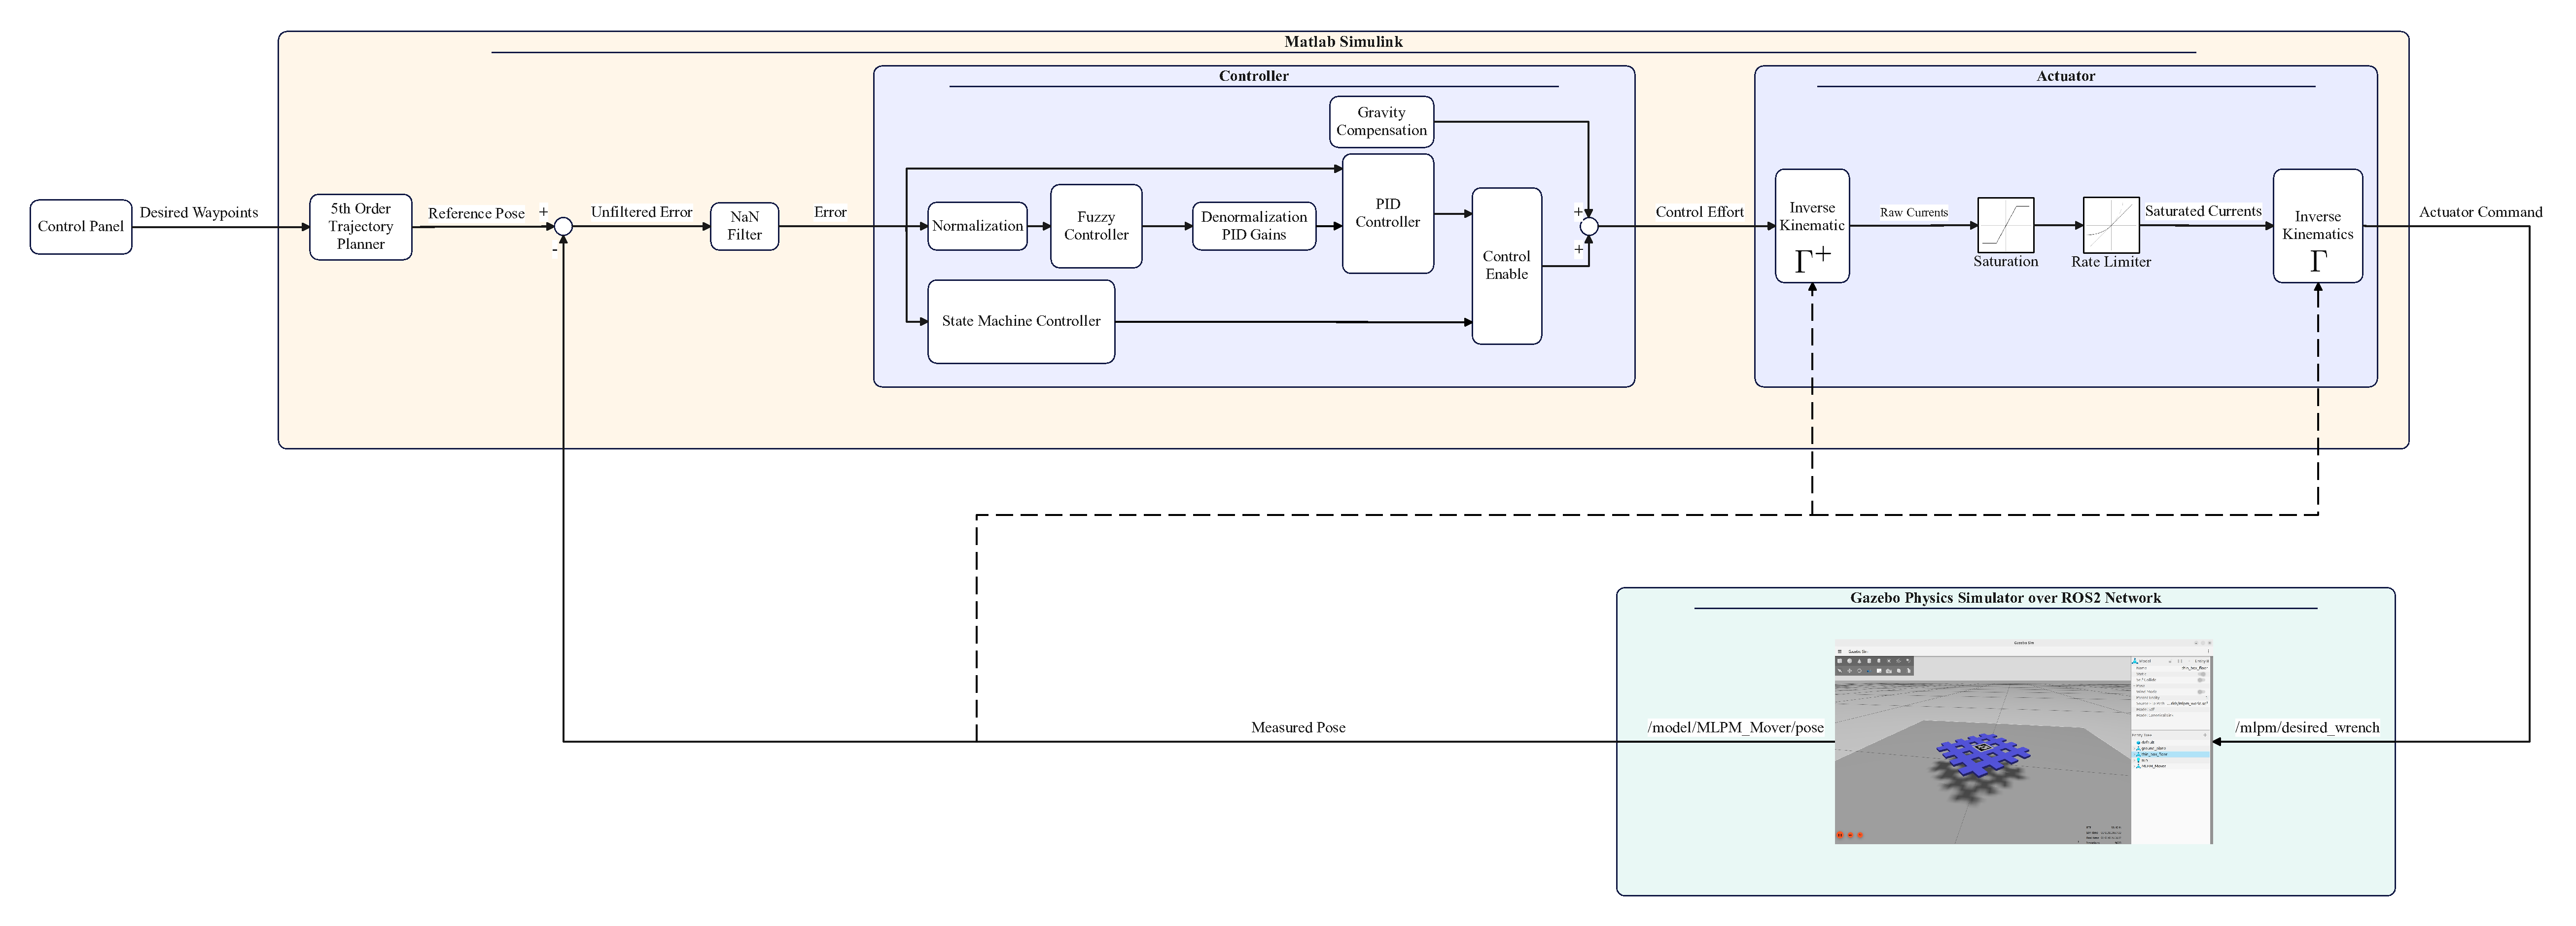
\includegraphics[width=0.95\textwidth]{img/system-overview.pdf}
	\caption{نمای کلی سیستم شبیه‌سازی و حلقه‌ی کنترل}
	\label{fig:method-system-overview}
\end{figure}

در نهایت، پس از استقرار یک سامانه‌ی کنترلی کامل، \textbf{تحلیل تکینگی سینماتیکی} (بخش \ref{sec:method-singularity}) بر روی ماتریس $\Gamma$ انجام می‌شود. در این تحلیل، با استفاده از تجزیه مقادیر تکین و یک جستجوی شبکه‌ای، پیکربندی‌هایی که در آن‌ها سیستم دچار افت شدید قابلیت مانور یا ناپایداری عددی می‌شود شناسایی می‌گردند و علل فیزیکی یا مدلی آن‌ها آشکار می‌شود. نتایج این بخش، مبنایی برای طراحی مسیرهای ایمن و اجتناب از نواحی تکین در آزمایش‌های فصول بعد فراهم می‌کند.

بدین ترتیب، این فصل مسیر کامل ساخت شبیه‌ساز، از مدل‌سازی تا تحلیل نهایی را گام‌به‌گام پوشش می‌دهد و زمینه‌ی ارزیابی‌های تجربی فصل \ref{ch:results} را مهیا می‌سازد.


\section{مدل سیستم}
\label{sec:method-system-model}

	همان طور که در بخش های پیشین توضیح داده شد، ساختار سیستم $MLPM$ از دو بخش متحرک و ثابت تشکیل می شود که بخش متجرک حاوی آرایه‌ی هالباخ بوده و بخش ثابت، سیم پیچ ها را شامل می شود. برای مدل سازی این سیستم، لازم است در نظر داشته باشیم که هدف نهایی از طراحی این سیستم کنترل دقیق موقعیت و جهت گیری بخش متحرک است. بنابراین، از این پس منظور از Plant سیستم پیشنهاد شده، تنها بخش متحرک آن است و سیم پیچ ها به عنوان عملگر شناخته می شوند که به صورت مجزا درباره ی آن توضیح داده خواهد شد.
لازم به توضیح است که پارامتر ها و مدل های مورد استفاده در این بخش بر اساس سیستم طراحی شده در پژوهش \cite{RN10} تعریف شده اند.
در بخش اول از این قسمت، به توضیح مدل بخش متحرک سیستم خواهیم پرداخت.
\subsection{مدل سیستم متحرک}
\label{subsec:method-mover-model}
در این سیستم، به دلیل وجود نداشتن نیروهای اتلافی از جمله اصطکاک و با صرف نظر از مقاومت هوا، می توان سیستم را به عنوان یک جسم ساده و با در نظر گرفتن جرم و ممان های اینرسی آن مدل کرد. بنابراین، روابط دینامیکی زیر برای آن برقرار خواهد بود:
\begin{align}
	m \ddot{P_x} = F_x, \quad m \ddot{P_y} = F_y, \quad m \ddot{P_z} = F_z
	\label{eq:method-translational-eom}
\end{align}


\begin{align}
	I_{xx} \ddot{\alpha} = T_x, \quad I_{yy} \ddot{\beta} = T_y, \quad I_{zz} \ddot{\gamma} = T_z
	\label{eq:method-rotational-eom}
\end{align}


در نتیجه، با محاسبه ی ماتریس های حالت برای این سیستم به صورت زیر خواهیم داشت:
\begin{equation}
	\dot{x} = A x + B u + g
	\label{eq:method-state-dynamics}
\end{equation}
\begin{equation}
	y = C x + D u
	\label{eq:method-output}
\end{equation}

\begin{equation}
	A =
	\begin{bmatrix}
		0 & 1 & 0 & 0 & 0 & 0 & 0 & 0 & 0 & 0 & 0 & 0 \\
		0 & 0 & 0 & 0 & 0 & 0 & 0 & 0 & 0 & 0 & 0 & 0 \\
		0 & 0 & 0 & 1 & 0 & 0 & 0 & 0 & 0 & 0 & 0 & 0 \\
		0 & 0 & 0 & 0 & 0 & 0 & 0 & 0 & 0 & 0 & 0 & 0 \\
		0 & 0 & 0 & 0 & 0 & 1 & 0 & 0 & 0 & 0 & 0 & 0 \\
		0 & 0 & 0 & 0 & 0 & 0 & 0 & 0 & 0 & 0 & 0 & 0 \\
		0 & 0 & 0 & 0 & 0 & 0 & 0 & 1 & 0 & 0 & 0 & 0 \\
		0 & 0 & 0 & 0 & 0 & 0 & 0 & 0 & 0 & 0 & 0 & 0 \\
		0 & 0 & 0 & 0 & 0 & 0 & 0 & 0 & 0 & 1 & 0 & 0 \\
		0 & 0 & 0 & 0 & 0 & 0 & 0 & 0 & 0 & 0 & 0 & 0 \\
		0 & 0 & 0 & 0 & 0 & 0 & 0 & 0 & 0 & 0 & 0 & 1 \\
		0 & 0 & 0 & 0 & 0 & 0 & 0 & 0 & 0 & 0 & 0 & 0
	\end{bmatrix}
	\label{eq:method-A-matrix}
\end{equation}
\begin{equation}
	B =
	\begin{bmatrix}
		0 & 0 & 0 & 0 & 0 & 0 \\
		\frac{1}{m} & 0 & 0 & 0 & 0 & 0 \\
		0 & 0 & 0 & 0 & 0 & 0 \\
		0 & \frac{1}{m} & 0 & 0 & 0 & 0 \\
		0 & 0 & 0 & 0 & 0 & 0 \\
		0 & 0 & \frac{1}{m} & 0 & 0 & 0 \\
		0 & 0 & 0 & 0 & 0 & 0 \\
		0 & 0 & 0 & \frac{1}{I_{xx}} & 0 & 0 \\
		0 & 0 & 0 & 0 & 0 & 0 \\
		0 & 0 & 0 & 0 & \frac{1}{I_{yy}} & 0 \\
		0 & 0 & 0 & 0 & 0 & 0 \\
		0 & 0 & 0 & 0 & 0 & \frac{1}{I_{zz}}
	\end{bmatrix}
	\label{eq:method-B-matrix}
\end{equation}
\begin{equation}
	g =
	\begin{bmatrix}
		0 \\ 0 \\ 0 \\ 0 \\ 0 \\ -g \\ 0 \\ 0 \\ 0 \\ 0 \\ 0 \\ 0
	\end{bmatrix}
	\label{eq:method-g-vector}
\end{equation}
\begin{equation}
	C = I_{12}, \quad
	D = 0_{12 \times 6}
	\label{eq:method-C-D}
\end{equation}


پارامتر های مورد استفاده در سیستم مورد دارای مقادیر زیر است:
\begin{align}
	m = 6.6 \text{ kg}, \quad g = 9.81 \text{m/s}^2
	\label{eq:method-mass-gravity}
\end{align}
\begin{align}
	I_{xx} = 0.059 \text{ kg}\cdot\text{m}^2, \quad
	I_{yy} = 0.059 \text{ kg}\cdot\text{m}^2, \quad
	I_{zz} = 0.12 \text{ kg}\cdot\text{m}^2
	\label{eq:method-inertia}
\end{align}

\subsection{مدل سیستم ثابت}
\label{subsec:method-stator-model}
عملگر سیستم که متشکل از 16 سیم پیچ که در آرایه ای 4 در 4 چیده شده اند می باشد، وظیفه ی اعمال نیرو و گشتاور تعیین شده توسط کنترلر را به متحرک بر عهده دارد. در صورتی که جریان الکتریکی گذرنده از هر سیم پیچ مشخص باشد، می توان نیرو و گشتاور برایند وارد بر متحرک را محاسبه کرد. البته به دلیل تعدد پارامتر ها و محدودیت های شبیه سازی، در این قسمت با استفاده از روش های تحلیلی، معادلاتی بر اساس داده های به دست آمده برای سیستم مورد نظر شناسایی شده است که در ادامه به شرح آنها خواهیم پرداخت.
\begin{enumerate}
	\item\textbf{ موقعیت سیم پیچ ها در دستگاه مختصات مرجع:}
	
	اولین مولفه ای که در این سیستم تعریف می شود، محل قرار گیری هر یک از سیم پیچ ها می باشد. در این مرحله، با در نظر گرفتن ابعاد سیم پیچ ها برابر با $\tau$ و تعداد سطر و ستون آرایه، محل قرار گیری مرکز هر یک مشخص می شود.  
	% Define Grid Parameters
	\begin{align}
		n_{\text{rows}} &= 4, \quad n_{\text{cols}} = 4
		\label{eq:method-grid-params}
	\end{align}
	% Position Calculation for Each Coil
	\begin{align}
		x_{\text{center}, j} &= (j - 1) \cdot \tau - \frac{(n_{\text{cols}} - 1) \cdot \tau}{2}, \quad j = 1, \dots, n_{\text{cols}}
		\label{eq:method-xcenter}
	\end{align}
	\begin{align}
		y_{\text{center}, i} &= (i - 1) \cdot \tau - \frac{(n_{\text{rows}} - 1) \cdot \tau}{2}, \quad i = 1, \dots, n_{\text{rows}}
		\label{eq:method-ycenter}
	\end{align}
	\begin{align}
		z_{\text{center}} &= 0
		\label{eq:method-zcenter}
	\end{align}
	در نهایت، موقعیت تمام سیم پیچ ها در سه راستای $x$، $y$ و $z$ در یک ماتریس ذخیره برای استفاده در مراحل بعد ذخیره می شود.
	% Final Position Matrix
	\begin{align}
		\mathbf{positions} =
		\begin{bmatrix}
			x_{\text{center}, 1}, y_{\text{center}, 1}, z_{\text{center}} \\
			x_{\text{center}, 2}, y_{\text{center}, 2}, z_{\text{center}} \\
			\vdots & \vdots & \vdots \\
			x_{\text{center}, n_{\text{cols}}}, y_{\text{center}, n_{\text{rows}}}, z_{\text{center}}
		\end{bmatrix}
		\label{eq:method-position-matrix}
	\end{align}
	
	\item\textbf{ موقعیت سیم پیچ ها در دستگاه مختصات متحرک:}
	
	برای محاسبه نیرو و گشتاور، نیاز به دانستن فاصله ی دقیق سیم پیچ مورد بررسی تا موقعیت متحرک وجود دارد. بنابراین، با اندازه گیری مختصات متحرک و استفاده از موقعیت های تعیین شده هر سیم پیچ، می توان بردار فاصله این دو را در دستگاه مختصات مبدا به دست آورد.
	% Corrected Position and Distance Calculations
	\begin{align}
		\mathbf{c^{m}} &= R 
		\begin{bmatrix}
			x_{\text{coil}} - x_m \\
			y_{\text{coil}} - y_m \\
			z_{\text{coil}} - z_m
		\end{bmatrix}
		\label{eq:method-cm-vector}
	\end{align}
	که در آن R ماتریس دوران تبدیل مختصات متحرک به دستگاه مختصات مبدا می باشد:
	\begin{align}
		R = R_z^T R_y^T R_x^T
		\label{eq:method-rotation-matrix-order}
	\end{align}
	% Rotation Matrices
	\begin{align}
		R_x =
		\begin{bmatrix}
			1 & 0 & 0 \\
			0 & \cos(\alpha_{\text{rotation}}) & -\sin(\alpha_{\text{rotation}}) \\
			0 & \sin(\alpha_{\text{rotation}}) & \cos(\alpha_{\text{rotation}})
		\end{bmatrix}
		\label{eq:method-Rx}
	\end{align}
	\begin{align}
		R_y =
		\begin{bmatrix}
			\cos(\beta_{\text{rotation}}) & 0 & \sin(\beta_{\text{rotation}}) \\
			0 & 1 & 0 \\
			-\sin(\beta_{\text{rotation}}) & 0 & \cos(\beta_{\text{rotation}})
		\end{bmatrix}
		\label{eq:method-Ry}
	\end{align}
	\begin{align}
		R_z =
		\begin{bmatrix}
			\cos(\gamma_{\text{rotation}}) & -\sin(\gamma_{\text{rotation}}) & 0 \\
			\sin(\gamma_{\text{rotation}}) & \cos(\gamma_{\text{rotation}}) & 0 \\
			0 & 0 & 1
		\end{bmatrix}
		\label{eq:method-Rz}
	\end{align}
	\item \textbf{محاسبه نیرو:}
	
	با در اختیار داشتن $c^{m}$، می توان بر اساس رابطه شناسایی شده به صورت زیر نیروی برایند ناشی از جریان های الکتریکی I را محاسبه کرد. 
	\begin{align}
		F_x &= K_x \cos(\eta_x) \sin(\eta_y) \\
		F_y &= K_y \sin(\eta_x) \cos(\eta_y) \\
		F_z &= K_z \sin(\eta_x) \sin(\eta_y)
		\label{eq:method-force-components}
	\end{align}
	که پارامتر های استفاده شده در این رابطه به صورت زیر است:
	
	\begin{align}
		\eta_x &= \frac{\pi}{\tau} \cdot c^{m}_1, \quad 
		\eta_y = \frac{\pi}{\tau} \cdot c^{m}_2
		\label{eq:method-eta}
	\end{align}
	% Force Components
	\begin{align}
		K_x &= \alpha_x e^{\beta_k \cdot c^{m}_3}, \quad
		K_y = \alpha_y e^{\beta_k \cdot c^{m}_3}, \quad
		K_z = \alpha_z e^{\beta_k \cdot c^{m}_3}
		\label{eq:method-Kfactors}
	\end{align}
	\item \textbf{محاسبه گشتاور:}
	
	محاسبه ی گشتاور ناشی از هر سیم پیچ با استفاده از نیرو های محاسبه شده انجام می شود. با این تفاوت که علاوه بر آن، نیاز به محاسبه ی طول بازوی موثر نیز هست و با توجه به آنکه در این سیستم، بازوی فیزیکی وجود ندارد، لازم است طی محاسباتی این مقادیر محاسبه شوند. بنابراین خواهیم داشت:
	
	% Effective Radius Calculations
	\begin{align}
		r_{\text{eff},x1} &= c^{m}_1 - m_1 \tan(n c^{m}_1 + \frac{\pi}{2}) \\
		r_{\text{eff},x2} &= c^{m}_1 - m_2 \tan(n c^{m}_1 + \frac{\pi}{2}) \\
		r_{\text{eff},y1} &= c^{m}_2 - m_1 \tan(n c^{m}_2 + \frac{\pi}{2}) \\
		r_{\text{eff},y2} &= c^{m}_2 - m_2 \tan(n c^{m}_2 + \frac{\pi}{2}) \\
		r_{\text{eff},z1} &= -c^{m}_3 + \alpha_{rz} \\
		r_{\text{eff},z2} &= -c^{m}_3 + \alpha_{rz}
		\label{eq:method-effective-arms}
	\end{align}
	که در آن:
	\begin{align}
		m_1 &= \alpha_{m1} \cdot c^{m}_3 + \beta_{m1} \\
		m_2 &= \alpha_{m2} \cdot c^{m}_3 + \beta_{m2}
		\label{eq:method-m-params}
	\end{align}
	و
	\begin{align}
		n &= \frac{\pi}{\tau}
		\label{eq:method-n-param}
	\end{align}
	آنگاه، مقادیر گشتاور به صورت زیر محاسبه می شوند:
	% Torque Components
	\begin{align}
		T_x &= r_{\text{eff},y1} F_z - r_{\text{eff},z1} F_y \\
		T_y &= -r_{\text{eff},x1} F_z + r_{\text{eff},z2} F_x \\
		T_z &= r_{\text{eff},x2} F_y - r_{\text{eff},y2} F_x
		\label{eq:method-torque-components}
	\end{align}
	
	\item \textbf{ماتریس $\Gamma$}
	
	در نهایت، پس از محاسبه ی روابط نیرو و گشتاور، می توان آنها را در یک ماتریس با نماد $\Gamma$ تعریف کرد که این ماتریس شامل تمام اطلاعات لازم برای محاسبه ی نیرو و گشتاور ناشی از گذر جریان در هر یک از سیم پیچ ها می باشد. این ماتریس به صورت زیر تعریف می شود:
	% Final Gamma Matrix
	\begin{align}
		\mathbf{\Gamma} =
		\begin{bmatrix}
			F_x \\ F_y \\ F_z \\ T_x \\ T_y \\ T_z
		\end{bmatrix}
		\label{eq:method-Gamma-def}
	\end{align}
	و با در اختیار داشتن این ماتریس، مقدار پیچش\footnote{Wrench} ناشی از آن از ضرب ماتریسی زیر به دست می آید.
	\begin{equation}
		w_{m_{net}} = [w_{m_1}, w_{m_2}, \dots, w_{m_n}] [I_1, I_2, \dots, I_n]^T = \Gamma(\vec{c}_m) I,
		\label{eq:method-wrench-net}
	\end{equation}
	
	
\end{enumerate}
	
	پارامتر های استفاده شده برای این سیستم در جدول زیر نمایش داده شده اند:
	\begin{table}[htbp]
		\centering
		\begin{tabular}{|c|c|}
			\hline
			\textbf{Parameter} & \textbf{Value} \\
			\hline
			$\tau$ & $0.0508$ \\
			$\beta_k$ & $-87.14$ \\
			$\alpha_x$ & $3.9021$ \\
			$\alpha_y$ & $3.9021$ \\
			$\alpha_z$ & $5.5209$ \\
			$\alpha_{m1}$ & $-0.0715$ \\
			$\alpha_{m2}$ & $-0.1046$ \\
			$\beta_{m1}$ & $-0.123$ \\
			$\beta_{m2}$ & $-0.0203$ \\
			$\alpha_{rz}$ & $-0.0146$ \\
			$n_{\text{rows}}$ & $4$ \\
			$n_{\text{cols}}$ & $4$ \\
			$dT$ & $0.01$ \\
			$Mass$ & $6.6$ \\
			\hline
		\end{tabular}
		\caption{جدول پارامترهای مدل سیستم}
		\label{tab:method-parameters}
	\end{table}
	
	\subsection{محاسبه وارون ماتریس $\Gamma$}
	\label{subsec:method-pinv}
	در صورتی که بخواهیم با در اختیار داشتن مقدار پیچش (گشتاور و نیروی) مورد نیاز، جریان‌های سیم‌پیچ‌ها را محاسبه کنیم، باید از وارون ماتریس $\Gamma$ استفاده شود. اما از آنجا که این ماتریس غیرمربعی است و سیستم دارای درجات آزادی بیشتری نسبت به متغیرهای کنترل است  برای مینیمم کردن نرم جریان (مصرف حداقل انرژی)، از وارون شبه‌مورس-پنروز 
	
	استفاده می‌شود.
	\footnote{Moore-Penrose Pseudoinverse}
	اگرچه فرمول تحلیلی وارون راست به صورت $I = \Gamma^T (\Gamma \Gamma^T)^{-1} w_{m,\text{net}}$ تعریف می‌شود، اما در پیاده‌سازی‌های نرم‌افزاری (مانند نرم‌افزار MATLAB) استفاده مستقیم از این رابطه به دلیل مشکلات پایداری عددی و احتمال نزدیک شدن ماتریس $\Gamma \Gamma^T$ به حالت تکین (Singular)، توصیه نمی‌شود. به همین دلیل، برای محاسبه دقیق‌تر و پایدارتر وارون شبه‌ماتریس، از الگوریتم تجزیه مقادیر منفرد SVD
	\footnote{
		Singular Values Decomposition}
	استفاده می‌گردد.
	
	در این روش، ابتدا ماتریس $\Gamma$ به سه ماتریس مجزا تجزیه می‌شود:
	\begin{equation}
		\Gamma = U \Sigma V^T
		\label{eq:method-svd}
	\end{equation}
	که در آن $U$ و $V$ ماتریس‌های متعامد هستند و $\Sigma$ یک ماتریس قطری شامل مقادیر منفرد \footnote{Singular Values} سیستم، یعنی $\sigma_i$ است. سپس وارون شبه‌مورس-پنروز ($\Gamma^+$) به شکل زیر محاسبه می‌شود:
	\begin{equation}
		\Gamma^+ = V \Sigma^+ U^T
		\label{eq:method-pseudoinverse-svd}
	\end{equation}
	که در آن ماتریس $\Sigma^+$ از ترانهاده کردن ماتریس $\Sigma$ و معکوس کردن درایه‌های غیرصفر آن به صورت زیر بدست می‌آید:
	\begin{equation}
		\sigma^+_i = 
		\begin{cases} 
			\frac{1}{\sigma_i} & \text{ اگر } \sigma_i > \epsilon \\ 
			0 & \text{ اگر } \sigma_i \leq \epsilon 
		\end{cases}
		\label{eq:method-sigma-pinv}
	\end{equation}
	
	در نهایت، بردار جریان بهینه از طریق رابطه زیر محاسبه می‌شود:
	\begin{equation}
		I = \Gamma^+ w_{m,\text{net}}
		\label{eq:method-optimal-current}
	\end{equation}
	
	مزیت اصلی استفاده از الگوریتم SVD (مانند دستور \texttt{pinv} در متلب) این است که با تعریف یک حد آستانه ($\epsilon$)، از تقسیم بر مقادیر منفرد بسیار کوچک (که نشان‌دهنده تکینگی یا بدشرط بودن ماتریس در موقعیت‌های خاص هستند) جلوگیری شده و از تولید جریان‌های بی‌نهایت و غیرفیزیکی جلوگیری به عمل می‌آید.
	
	\subsection{تخصیص سیگنال کنترلی و شبیه‌سازی محدودیت‌های سخت‌افزاری}
	\label{subsec:method-allocation}
	
	در پیاده‌سازی فیزیکی سیستم، پس از آنکه کنترل‌کننده برآیند نیرو و گشتاور مطلوب\footnote{Desired Wrench} را محاسبه می‌نماید، این مقادیر باید به سیگنال‌های قابل فهم برای سخت‌افزار تبدیل شوند. برای این منظور، از بلوک وارون ماتریس نگاشت ($\Gamma^\dagger$) استفاده می‌شود که پیچش مطلوب را به جریان‌های الکتریکی مرجع برای تخصیص به ۱۶ سیم‌پیچ\footnote{Coils} سیستم تبدیل می‌کند. در دستگاه واقعی، این جریان‌ها مستقیماً به مدارهای درایور ارسال شده و با عبور از سیم‌پیچ‌ها، نیروی محرکه نهایی را بر روی بخش متحرک اعمال می‌کنند.
	
	با این وجود، در محیط شبیه‌ساز به دلیل عدم حضور سخت‌افزار و مدارهای الکتریکی، نیازمند رویکردی جایگزین برای مدل‌سازی دقیق این فرآیند هستیم. از آنجا که سیستم‌های فیزیکی همواره دارای محدودیت‌های ذاتی در تأمین توان و جریان هستند، اعمال مستقیم پیچش ایده‌آلِ محاسبه‌شده توسط کنترل‌کننده به شبیه‌ساز فیزیکی، می‌تواند به نتایجی غیرواقعی و خارج از توان عملیاتی دستگاه منجر شود. 
	
	برای رفع این چالش و نزدیک کردن رفتار شبیه‌ساز به واقعیت فیزیکی، یک ساختار جبران‌ساز و محدودکننده به معماری سیستم افزوده شده است (همان‌طور که در بلوک‌دیاگرام شبیه‌ساز مشخص است). در این ساختار، ابتدا پیچش مطلوب ($W_{des}$) با استفاده از معادلات سینماتیک معکوس به جریان‌های خام ($I_{raw}$) نگاشت می‌شود:
	\begin{equation}
		I_{raw} = \Gamma^\dagger(\mathbf{x}) W_{des}
		\label{eq:method-raw-current}
	\end{equation}
	که در آن $\mathbf{x}$ بردار موقعیت فعلی جسم متحرک است. 
	
	سپس، برای مدل‌سازی محدودیت‌های سخت‌افزاری، این جریان‌های خام از یک بلوک اشباع\footnote{Saturation Block} عبور داده می‌شوند. بر اساس مشخصات فنی و مقالات مرجع سیستم، حداکثر جریان مجاز عبوری از هر سیم‌پیچ برابر با $9$ آمپر در نظر گرفته شده است. بنابراین، جریان‌های اشباع‌شده ($I_{sat}$) به شکل زیر محاسبه می‌گردند:
	\begin{equation}
		I_{sat} = \text{sat}(I_{raw}, -I_{max}, I_{max}), \quad I_{max} = 9 \text{ A}
		\label{eq:method-current-saturation}
	\end{equation}
	
	در نهایت، برای محاسبه نیروی خالصی که واقعاً به جسم اعمال خواهد شد، این جریان‌های محدودشده مجدداً از طریق ماتریس سینماتیک مستقیم ($\Gamma$) به فضای نیرو و گشتاور بازگردانده می‌شوند:
	\begin{equation}
		W_{act} = \Gamma(\mathbf{x}) I_{sat}
		\label{eq:method-actual-wrench}
	\end{equation}
	پیچش نهایی و واقعی محاسبه‌شده ($W_{act}$)، به عنوان نیروی محرکه سیستم، جهت شبیه‌سازی دینامیکِ حرکت به محیط ROS2 ارسال (Publish) می‌شود. 
	
	علاوه بر این، به منظور حفظ یکپارچگی معماری نرم‌افزار و تسهیل فرآیند گذار از فاز شبیه‌سازی به پیاده‌سازی فیزیکی، مقادیر جریان‌های اشباع‌شده ($I_{sat}$) نیز در یک تاپیک مجزا در شبکه ROS2 منتشر می‌گردند. این معماری تضمین می‌کند که کدهای توسعه‌یافته در بستر ROS2، بدون نیاز به تغییرات ساختاری، قادر خواهند بود در آینده برای تحریک درایورهای سخت‌افزار واقعی مورد استفاده قرار گیرند.
	
	
	\section{توسعه بستر شبیه‌سازی در چارچوب \lr{ROS 2} و \lr{Gazebo}}
	\label{sec:method-sim-env}
	
	به منظور ارزیابی عملکرد و اعتبارسنجی الگوریتم‌های کنترلی موتور مسطح با شناوری مغناطیسی (\lr{MLPM}) پیش از پیاده‌سازی عملی، یک محیط شبیه‌سازی فیزیکی یکپارچه و با دقت بالا توسعه یافته است. این شبیه‌ساز بر پایه سیستم‌عامل رباتیک نسخه ۲ (\lr{ROS 2}) و شبیه‌ساز پیشرفته \lr{Gazebo Harmonic} بنا شده است. هدف اصلی از توسعه این بستر، ایجاد یک محیط دینامیکی است که در آن مشخصات سینماتیکی و اینرسیایی پلتفرم معلق به دقت تعریف شده، فرامین کنترلی به صورت نیرو و گشتاور به سیستم اعمال گردیده و متغیرهای حالت به صورت بی‌درنگ (\lr{Real-time}) استخراج و به کنترل‌کننده مرکزی (پیاده‌سازی‌شده در نرم‌افزار \lr{MATLAB}) ارسال شوند. ساختار نرم‌افزاری این شبیه‌ساز در قالب یک بسته (\lr{Package}) مستقل با نام \lr{description} سازماندهی شده است که در آن، اسکریپت‌های \lr{CMakeLists.txt} و \lr{setup.py} وظیفه مدیریت وابستگی‌ها، کامپایل و نصب فایل‌های پیکربندی (نظیر \lr{URDF} و فایل‌های \lr{Launch}) را بر عهده دارند.
	
	\subsection{مدل‌سازی فیزیکی و هندسی سیستم متحرک}
	\label{subsec:method-urdf-model}
	ساختار فیزیکی پلتفرم متحرک با بهره‌گیری از استاندارد \lr{URDF} و استفاده از ماکروهای \lr{Xacro} در فایل \lr{mlpm.urdf} مدل‌سازی شده است. در این ساختار، پلتفرم متحرک به عنوان یک پیوند شناور (\lr{Floating Link}) با شناسه \lr{base\_link} در فضای شبیه‌سازی تعریف می‌گردد. پارامترهای اینرسی سیستم با تطابق کامل بر مدل فیزیکی واقعی تعیین شده‌اند؛ به گونه‌ای که جرم پلتفرم برابر با $m = 6.6$ کیلوگرم و درایه‌های اصلی تانسور اینرسی به ترتیب $I_{xx} = 0.06$، $I_{yy} = 0.06$ و $I_{zz} = 0.12$ کیلوگرم در متر مربع لحاظ شده‌اند. 
	
	برای نمایش بصری (\lr{Visual Geometry}) مدل در محیط‌های \lr{Gazebo} و \lr{RViz}، از فایل‌های شبکه (\lr{Mesh}) با فرمت \lr{STL} مربوط به آرایه هالباخ (\lr{Halbach Array}) با ضریب مقیاس $0.001$ استفاده شده است تا جزئیات ظاهری پلتفرم حفظ گردد. با این حال، به منظور بهینه‌سازی بار محاسباتی موتور فیزیک، هندسه برخورد (\lr{Collision Geometry}) به یک مکعب‌مستطیل ساده با ابعاد $0.2286 \times 0.2286 \times 0.013$ متر تقلیل یافته است تا محاسبات مربوط به تشخیص تداخل (\lr{Collision Detection}) با بالاترین سرعت ممکن انجام پذیرد.
	
	\subsection{پیکربندی موتور فیزیک و شرایط مرزی محیط}
	\label{subsec:method-physics-config}
	محیط فیزیکی شبیه‌سازی در قالب فایل \lr{mlpm\_world.sdf} پیکربندی شده است. برای حل معادلات دیفرانسیل حاکم بر دینامیک جسم صلب، از موتور فیزیک \lr{DART} استفاده شده است که پایداری عددی مطلوبی در شبیه‌سازی سیستم‌های شناور ارائه می‌دهد. به منظور تضمین دقت محاسبات دینامیکی، به ویژه در حضور نیروهای تحریک و پاسخ‌های فرکانس بالای سیستم، بیشینه گام زمانی شبیه‌سازی (\lr{Max Step Size}) روی مقدار $\Delta t = 0.005$ ثانیه تنظیم گردیده است. 
	
	همچنین، بردار شتاب گرانش به صورت $g = \begin{bmatrix} 0 & 0 & -9.8 \end{bmatrix}^T$ متر بر مجذور ثانیه در محیط اعمال شده است. از منظر مدل‌های استاتیک محیطی، یک صفحه مرجع (\lr{Ground Plane}) با ضریب اصطکاک استاتیکی و دینامیکی $\mu = 0.8$ به همراه یک کف‌پوش با ضخامت اندک (\lr{Thin Box Floor}) در دنیای شبیه‌سازی تعریف شده‌اند تا شرایط مرزی فیزیکی برای حالت استراحت پلتفرم فراهم گردد.
	
	\subsection{استخراج متغیرهای حالت و اعمال فرامین کنترلی}
	\label{subsec:method-state-feedback}
	بسته شدن حلقه کنترل نیازمند دریافت بازخورد دقیق از وضعیت سیستم و اعمال متقابل تلاش کنترلی (\lr{Control Effort}) است. برای این منظور، از افزونه‌های استاندارد \lr{Gazebo} در فایل \lr{mlpm.gazebo} بهره گرفته شده است:
	\begin{itemize}
		\item \textbf{استخراج موقعیت (\lr{State Feedback}):} افزونه \lr{PosePublisher} به مدل متصل شده است که وظیفه محاسبه و انتشار موقعیت و جهت‌گیری (\lr{Pose}) پلتفرم را نسبت به دستگاه مختصات مرجع با فرکانس $60$ هرتز بر عهده دارد.
		\item \textbf{اعمال ورودی‌های کنترلی (\lr{Wrench Application}):} از آنجا که سیستم کنترلی در فضای خارج از \lr{Gazebo} عمل می‌کند، افزونه \lr{ApplyLinkWrench} پیکربندی شده است. این افزونه سیگنال‌های نیرو و گشتاور محاسبه‌شده را از طریق تاپیک \lr{/world/mlpm\_world/wrench} دریافت کرده و مستقیماً به مرکز جرم \lr{base\_link} اعمال می‌نماید.
	\end{itemize}
	علاوه بر موارد فوق، به منظور جلوگیری از بروز تکینگی‌های عددی و ناپایداری‌های فیزیکی در حین شبیه‌سازی، سرعت‌های خطی و زاویه‌ای پلتفرم به ترتیب به مقادیر بیشینه $10$ متر بر ثانیه و $5$ رادیان بر ثانیه محدود شده‌اند.
	
	\subsection{مدیریت ارتباطات، همگام‌سازی و رله سیگنال‌های گسسته}
	\label{subsec:method-ros-integration}
	هماهنگ‌سازی و اجرای همزمان گره‌های پردازشی (\lr{Nodes}) از طریق فایل‌های راه‌انداز 
	\lr{sim\_gazebo.launch.py} و \lr{spawn.launch.py} مدیریت می‌شود. پس از تنظیم مسیرهای مرجع (\lr{Resource Paths})، پلتفرم ربات در ارتفاع اولیه $Z = 4.0$ متر در محیط شبیه‌سازی بارگذاری (\lr{Spawn}) می‌گردد.
	
	هسته اصلی ارتباط بین شبیه‌ساز و شبکه \lr{ROS 2}، گره \lr{parameter\_bridge} است که تبدیل و مسیریابی پیام‌ها را بر عهده دارد. از طریق این پل ارتباطی، داده‌های حیاتی نظیر سیگنال ساعت شبیه‌ساز (\lr{Clock}) برای همگام‌سازی زمان و همچنین موقعیت مدل به شبکه ارسال می‌شوند. تنظیمات کیفیت سرویس (\lr{QoS}) برای این تاپیک‌ها به صورت \lr{Reliable} با عمق تاریخچه محدود در نظر گرفته شده است تا از افت بسته‌های داده جلوگیری شود.
	
	یکی از چالش‌های اساسی در شبیه‌سازی سیستم‌های کنترل دیجیتال متصل به یک محیط فیزیکی پیوسته، نحوه اعمال سیگنال‌های کنترلی گسسته است. برای رفع این چالش، گره‌های سفارشی با عناوین \lr{wrench\_zoh\_relay} و \lr{wrench\_sequencer} توسعه یافته‌اند. این گره‌ها وظیفه دارند سیگنال‌های نیرو و گشتاور ارسال شده از سوی کنترل‌کننده را دریافت کرده و بر اساس منطق نگهدارنده مرتبه صفر (\lr{Zero-Order Hold})، آن‌ها را تا دریافت نمونه بعدی به صورت پیوسته و پایدار به محیط \lr{Gazebo} تزریق کنند. این معماری تضمین می‌کند که فرآیند شبیه‌سازی تطابق بالایی با رفتار واقعی سیستم‌های کنترل نمونه‌برداری‌شده داشته باشد.
	
	\section{طراحی و پیاده‌سازی کنترل‌کننده \lr{Fuzzy PID}}
	\label{sec:method-control-design}
	
	در این بخش، به بررسی دقیق معماری کنترلی توسعه‌یافته برای تنظیم وضعیت و موقعیت شبیه‌ساز  سیستم موتور صفحه ای پرداخته می‌شود. متغیرهای کنترلی در این سیستم شامل شش درجه آزادی ($X, Y, Z$ و زوایای رول، پیچ و یاو) است و متغیرهای سرعت به عنوان هدف کنترلی در نظر گرفته نشده‌اند. با توجه به چالش‌های تنظیم ضرایب کلاسیک در تعامل با موتور فیزیک \lr{Gazebo}، از یک رویکرد فازی برای تنظیم پویای ضرایب استفاده شده است.
	
	\subsection{چالش‌های کنترل کلاسیک و ضرورت گذر به منطق فازی}
	\label{subsec:method-classical-challenges}
	در مراحل ابتدایی توسعه، از کنترل‌کننده \lr{PID} کلاسیک با ضرایب ثابت استفاده گردید. با این حال، تنظیم (\lr{Tuning}) این ضرایب در محیط شبیه‌ساز با چالش‌های جدی مواجه شد. دینامیک غیرخطی سیستم، وجود نویزهای عددی ناشی از حل‌گر فیزیک \lr{DART} و تاخیرهای ذاتی در تبادل پیام‌های شبکه \lr{ROS 2} باعث می‌شد تا ضرایبی که برای یک نقطه کاری خاص تنظیم شده بودند، در مواجهه با تغییرات بزرگ در موقعیت یا اغتشاشات خارجی، عملکرد پایداری نداشته باشند. برای غلبه بر این محدودیت‌ها، یک کنترل‌کننده \lr{Fuzzy PID} طراحی شد تا با درک شرایط لحظه‌ای سیستم، ضرایب کنترلی را به صورت بلادرنگ تطبیق دهد.
	
	\subsection{معماری سیستم استنتاج فازی (\lr{FIS})}
	\label{subsec:method-fis-architecture}
	سیستم استنتاج فازی طراحی‌شده بر مبنای مدل تاکاگی-سوگنو (\lr{Takagi-Sugeno}) مرتبه صفر توسعه یافته است. در این ساختار، هدف استخراج ضرایب نرمالیزه‌شده‌ای است که رفتار تناسبی، انتگرال‌گیر و مشتق‌گیر را تعدیل می‌کنند.
	
	\subsubsection{ساختار و مبانی ریاضی کنترل‌کننده فازی (\lr{Structure and Mathematical Foundations of FIS})}
	\label{subsec:method-fuzzy-theory}
	
	به منظور تنظیم پیوسته و تطبیقی ضرایب کنترل‌کننده \lr{PID} در طول پرواز، از یک سیستم استنتاج فازی (\lr{Fuzzy Inference System - FIS}) استفاده شده است. با توجه به الزامات پیاده‌سازی بلادرنگ (\lr{Real-time}) در کنترل ربات‌ها و نیاز مبرم به یک سطح کنترلی هموار (\lr{Smooth Control Surface}) برای جلوگیری از نوسانات ناگهانی، این سیستم بر پایه توابع عضویت ورودی از نوع گوسی (\lr{Gaussian}) و خروجی‌های تک‌مقداری (\lr{Singleton}) طراحی شده است. از منظر مبانی تئوری، این ساختار معادل یک سیستم استنتاج ممدانی (\lr{Mamdani}) با خروجی سینگلتون و یا سیستم تاکاگی-سوگنو مرتبه صفر (\lr{Zero-Order Takagi-Sugeno}) است. دیاگرام کلی این ساختار و مسیر پردازش سیگنال‌ها در شکل \ref{fig:method-fuzzy-diagram} به تفصیل نشان داده شده است.
	
	\begin{figure}[htbp]
		\centering
		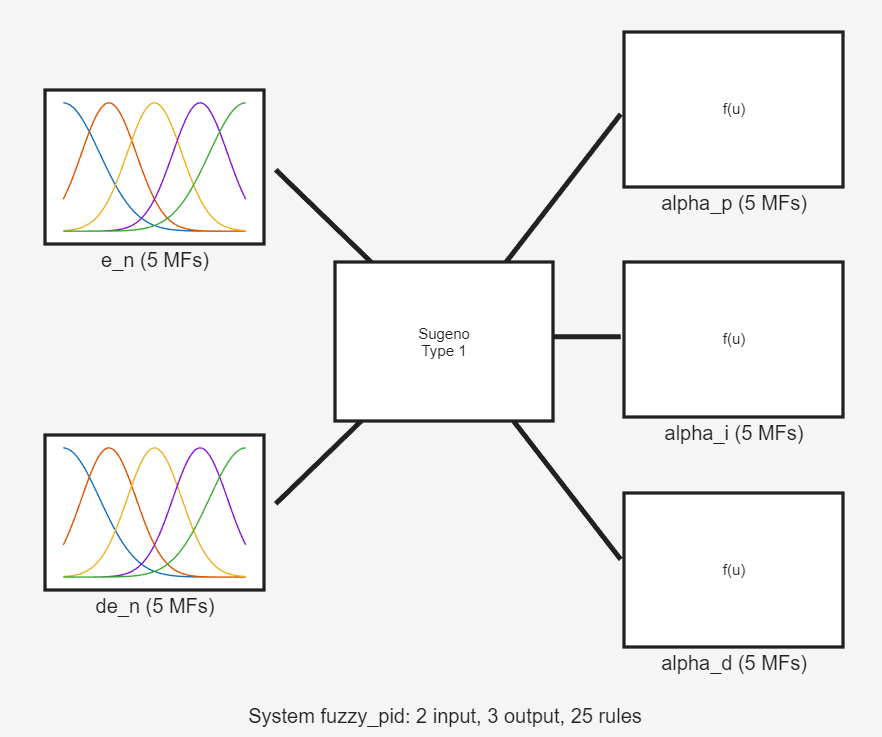
\includegraphics[width=0.7\linewidth]{img/fuzzy_diagram}
		\caption{ساختار منطق فازی، بلوک‌های پیش‌پردازش و مسیر پردازش سیگنال در کنترل‌کننده}
		\label{fig:method-fuzzy-diagram}
	\end{figure}
	
	\paragraph{پیش‌پردازش و مقیاس‌بندی ورودی‌ها (\lr{Preprocessing and Normalization})}
	پیش از آنکه سیگنال‌های خطا وارد هسته محاسباتی فازی شوند، نیاز به پیش‌پردازش دارند. در ابتدا، سیگنال‌های خطای واقعی مکان و مشتق آن توسط بلوک‌های اشباع (\lr{Saturation}) محدود می‌شوند. این کار از ورود مقادیر بسیار بزرگ (که ممکن است در لحظه شروع حرکت یا بروز اغتشاش شدید رخ دهند) به سیستم فازی جلوگیری می‌کند. سپس این سیگنال‌های محدود شده، با استفاده از ضریب نرمال‌سازی ($G_E$) به یک بازه استاندارد و بدون بعد $[-1, 1]$ نگاشت می‌شوند. اهمیت این فرآیند در آن است که باعث می‌شود سیستم فازی کاملاً مستقل از مقیاس فیزیکی و دینامیک خاص هر محور (انتقالی یا دورانی) عمل کند و بتوان از یک پایگاه قوانینِ واحد برای تمامی درجات آزادی کوادکوپتر استفاده نمود. 
	
	\paragraph{فازی‌سازی ورودی‌ها (\lr{Fuzzification})}
	در مرحله فازی‌سازی، مقادیر قطعیِ خطای نرمال‌شده ($e_n$) و تغییرات خطای نرمال‌شده ($de_n$) به درجات عضویت فازی تبدیل می‌شوند. فضای گفتمان (\lr{Universe of Discourse}) برای هر دو متغیر ورودی به پنج مجموعه فازی تقسیم شده است که عبارتند از: منفی بزرگ (\lr{NB})، منفی کوچک (\lr{NS})، صفر (\lr{Z})، مثبت کوچک (\lr{PS}) و مثبت بزرگ (\lr{PB}). 
	
	رابطه ریاضی تابع عضویت گوسی برای یک متغیر زبانی نظیر $A_i^j$ به صورت معادله (\ref{eq:method-gaussian-mf}) تعریف می‌گردد:
	
	\begin{equation} \label{eq:method-gaussian-mf}
		\mu_{A_i^j}(x_i) = \exp \left( -\frac{1}{2} \left( \frac{x_i - c_i^j}{\sigma_i^j} \right)^2 \right)
	\end{equation}
	
	که در این رابطه، $x_i \in \{e_n, de_n\}$ نشان‌دهنده متغیر ورودی قطعی، $c_i^j$ پارامتر تعیین‌کننده مرکز (میانگین) تابع عضویت، و $\sigma_i^j$ انحراف معیار (\lr{Standard Deviation}) آن است که میزان گستردگی تابع را مشخص می‌کند. مقادیر دقیق این پارامترها در جدول \ref{tab:method-input-mfs} ارائه شده است. 
	
	انتخاب توابع گوسی به جای توابع رایج‌تر مانند مثلثی یا ذوزنقه‌ای، تصمیمی آگاهانه بوده است. توابع گوسی در تمامی نقاط مشتق‌پذیر و پیوسته هستند. این ویژگی باعث می‌شود تغییرات در خروجی فازی کاملاً نرم باشد و از اعمال هرگونه شوک یا پرش ناگهانی به عملگرهای فیزیکی در محیط شبیه‌ساز \lr{Gazebo} جلوگیری شود. شکل توابع عضویت ورودی در شکل \ref{fig:method-fuzzy-inputs} ترسیم شده است.
	
	\begin{table}[htbp]
		\centering
		\caption{پارامترهای توابع عضویت گوسی برای متغیرهای ورودی خطا ($e_n$) و مشتق خطا ($de_n$)}
		\label{tab:method-input-mfs}
		\begin{tabular}{|c|c|c|c|}
			\hline
			\textbf{توصیف‌گر زبانی} & \textbf{نماد مجموعه فازی} & \textbf{مرکز تابع ($c$)} & \textbf{انحراف معیار ($\sigma$)} \\
			\hline
			منفی بزرگ & \lr{NB} & $-1$ & $0.4$ \\
			منفی کوچک & \lr{NS} & $-0.5$ & $0.3$ \\
			صفر & \lr{Z} & $0$ & $0.3$ \\
			مثبت کوچک & \lr{PS} & $0.5$ & $0.3$ \\
			مثبت بزرگ & \lr{PB} & $1$ & $0.4$ \\
			\hline
		\end{tabular}
	\end{table}
	
	\begin{figure}[htbp]
		\centering
		\subfloat[تابع عضویت ورودی خطای نرمال‌شده ($e_n$)]{
			\label{fig:method-input-mf-e}
			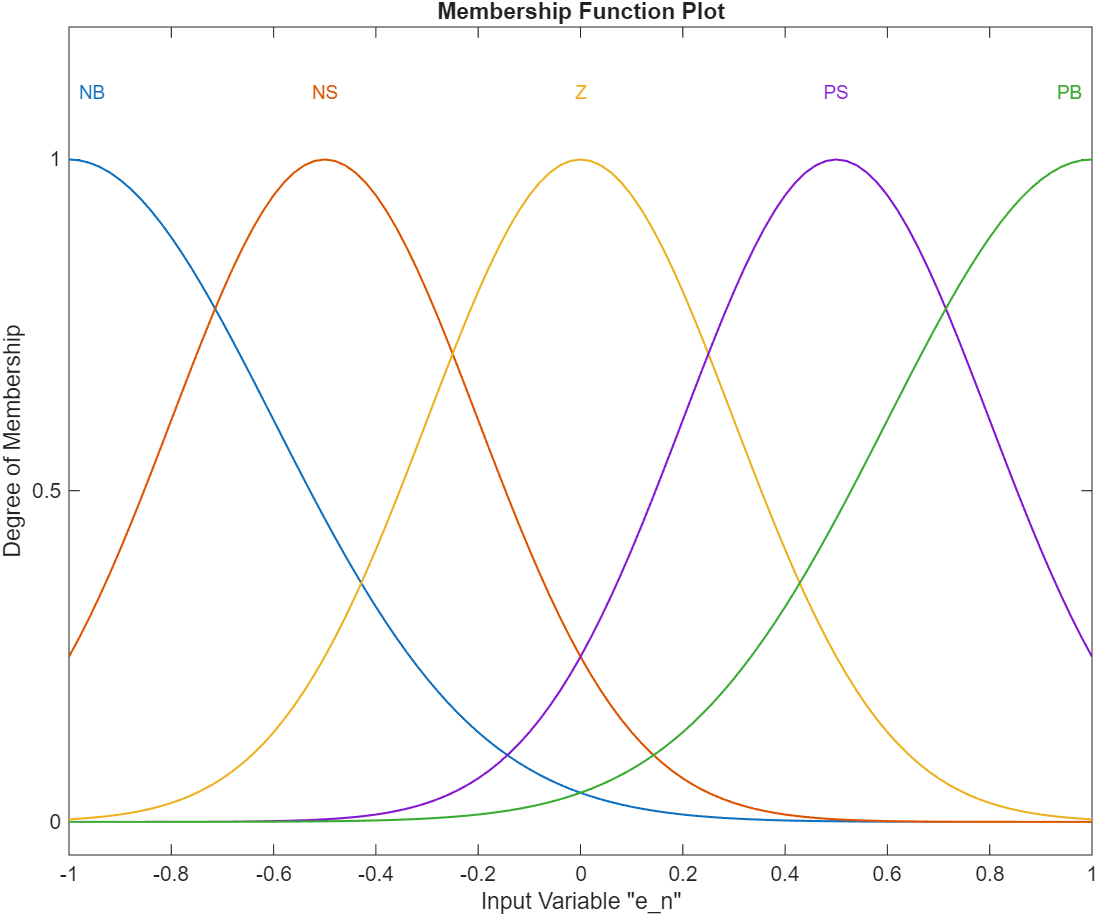
\includegraphics[width=0.45\textwidth]{img/fuzzy_input_mf_e_n}}
		\hspace{2mm}
		\subfloat[تابع عضویت ورودی مشتق خطای نرمال‌شده ($de_n$)]{
			\label{fig:method-input-mf-de}
			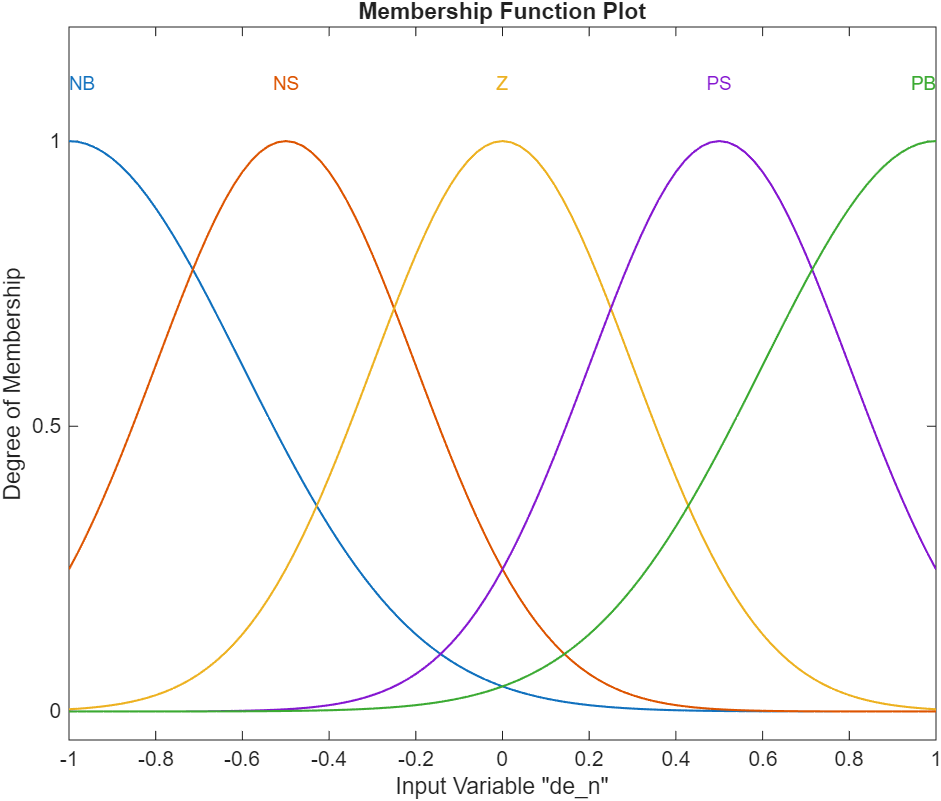
\includegraphics[width=0.45\textwidth]{img/fuzzy_input_mf_de_n}}
		\caption{توابع عضویت گوسی ورودی‌های سیستم استنتاج فازی}
		\label{fig:method-fuzzy-inputs}
	\end{figure}
	
	\paragraph{پایگاه قوانین و موتور استنتاج (\lr{Rule Base and Inference Engine})}
	هسته تصمیم‌گیری سیستم، پایگاه قوانینی متشکل از ۲۵ قانون فازی است که بر اساس تئوری کنترل کلاسیک و تجربه اپراتوری در تنظیم ضرایب \lr{PID} توسعه یافته است. فرم کلی قانون $k$-ام ($R^{(k)}$) به صورت ساختار شرطی زیر بیان می‌شود:
	
	\begin{equation} \label{eq:method-fuzzy-rule}
		R^{(k)} : \text{IF } e_n \text{ is } A_1^k \text{ \lr{AND} } de_n \text{ is } A_2^k \text{ THEN } \alpha_x \text{ is } B^k
	\end{equation}
	
	متغیرهای خروجی سیستم شامل $\alpha_p$، $\alpha_i$ و $\alpha_d$ هستند که مقادیر تنظیم‌کننده ضرایب تناسبی، انتگرال‌گیر و مشتق‌گیر را تعیین می‌کنند. این خروجی‌ها با توابع عضویت سینگلتون در پنج سطح توصیف می‌شوند: بسیار کم (\lr{VL})، کم (\lr{L})، متوسط (\lr{M})، زیاد (\lr{H}) و بسیار زیاد (\lr{VH}). 
	
	منطق حاکم بر این قوانین به گونه‌ای است که بهترین عملکرد دینامیکی حاصل شود. به عنوان مثال، زمانی که خطای سیستم مثبت بزرگ (\lr{PB}) است اما تغییرات خطا در محدوده صفر (\lr{Z}) قرار دارد، قانون فازی ضریب $\alpha_p$ را در حالت بسیار زیاد (\lr{VH}) قرار می‌دهد تا ربات با حداکثر توان به سمت نقطه هدف حرکت کند؛ اما به طور همزمان ضریب $\alpha_d$ کاهش می‌یابد تا از کند شدن پاسخ گذرا جلوگیری شود. در مقابل، هنگامی که خطا به صفر نزدیک می‌شود، $\alpha_p$ کاهش یافته و $\alpha_d$ افزایش می‌یابد تا نقش ترمزکننده داشته و مانع از فراجهش (\lr{Overshoot}) سیستم شود. این قوانین به تفکیک برای هر سه خروجی در جداول سه‌گانه \ref{tab:method-fuzzy-rules} ارائه شده‌اند.
	
	\begin{table}[htbp]
		\centering
		\caption{پایگاه قوانین (ماتریس ۲۵ تایی) برای تنظیم پویای ضرایب $\alpha_p$، $\alpha_i$ و $\alpha_d$}
		\label{tab:method-fuzzy-rules}
		
		% --- جدول آلفا P ---
		\vspace{0.3cm}
		\begin{tabular}{|c|c|c|c|c|c|}
			\hline
			\multicolumn{6}{|c|}{\textbf{قوانین خروجی تناسبی ($\alpha_p$)}} \\
			\hline
			$e_n \setminus de_n$ & \textbf{NB} & \textbf{NS} & \textbf{Z} & \textbf{PS} & \textbf{PB} \\
			\hline
			\textbf{NB} & VH & H & M & M & L \\
			\hline
			\textbf{NS} & H  & M & M & M & H  \\
			\hline
			\textbf{Z}  & M  & M & M & M & M  \\
			\hline
			\textbf{PS} & H  & M & M & M & H  \\
			\hline
			\textbf{PB} & VH & H & M & M & L \\
			\hline
		\end{tabular}
		
		% --- جدول آلفا I ---
		\vspace{0.6cm}
		\begin{tabular}{|c|c|c|c|c|c|}
			\hline
			\multicolumn{6}{|c|}{\textbf{قوانین خروجی انتگرالی ($\alpha_i$)}} \\
			\hline
			$e_n \setminus de_n$ & \textbf{NB} & \textbf{NS} & \textbf{Z} & \textbf{PS} & \textbf{PB} \\
			\hline
			\textbf{NB} & VL & VL & L & VL & VL \\
			\hline
			\textbf{NS} & L  & L  & M & L  & L  \\
			\hline
			\textbf{Z}  & M  & H  & H & H  & M  \\
			\hline
			\textbf{PS} & L  & L  & M & L  & L  \\
			\hline
			\textbf{PB} & VL & VL & L & VL & VL \\
			\hline
		\end{tabular}
		
		% --- جدول آلفا D ---
		\vspace{0.6cm}
		\begin{tabular}{|c|c|c|c|c|c|}
			\hline
			\multicolumn{6}{|c|}{\textbf{قوانین خروجی مشتقی ($\alpha_d$)}} \\
			\hline
			$e_n \setminus de_n$ & \textbf{NB} & \textbf{NS} & \textbf{Z} & \textbf{PS} & \textbf{PB} \\
			\hline
			\textbf{NB} & M  & H  & H & H  & M  \\
			\hline
			\textbf{NS} & H  & H  & M & H  & M  \\
			\hline
			\textbf{Z}  & H  & H  & M & H  & H  \\
			\hline
			\textbf{PS} & H  & H  & M & H  & M  \\
			\hline
			\textbf{PB} & M  & H  & H & H  & M  \\
			\hline
		\end{tabular}
	\end{table}
	
	
	برای ترکیب شرط‌ها در مقدمه هر قانون (عملگر \lr{AND})، از روش ضرب جبری (\lr{Algebraic Product}) استفاده شده است. این روش نسبت به عملگر مینیمم، رفتار تحلیلی بهتری از خود نشان می‌دهد. بنابراین، درجه تحقق (\lr{Firing Strength}) قانون $k$-ام ($f_k$) با توجه به رابطه (\ref{eq:method-firing-strength}) محاسبه می‌گردد:
	
	\begin{equation} \label{eq:method-firing-strength}
		f_k(e_n, de_n) = \mu_{A_1^k}(e_n) \cdot \mu_{A_2^k}(de_n)
	\end{equation}
	
	تاثیر جامع این ۲۵ قانون بر روی خروجی‌ها در قالب سطوح کنترلی سه‌بعدی در شکل \ref{fig:method-fuzzy-surfaces} به تصویر کشیده شده است. همانطور که در این شکل‌ها مشهود است، به دلیل استفاده از توابع گوسی و عملگر ضرب جبری، سطوح کنترلی تولید شده کاملاً هموار (\lr{Smooth}) و فاقد شکستگی هستند که شرط اصلی برای یک کنترل باثبات در رباتیک محسوب می‌شود.
	
	\begin{figure}[htbp]
		\centering
		\subfloat[سطح کنترلی تنظیم‌کننده تناسبی ($\alpha_p$)]{
			\label{fig:method-surface-alphap}
			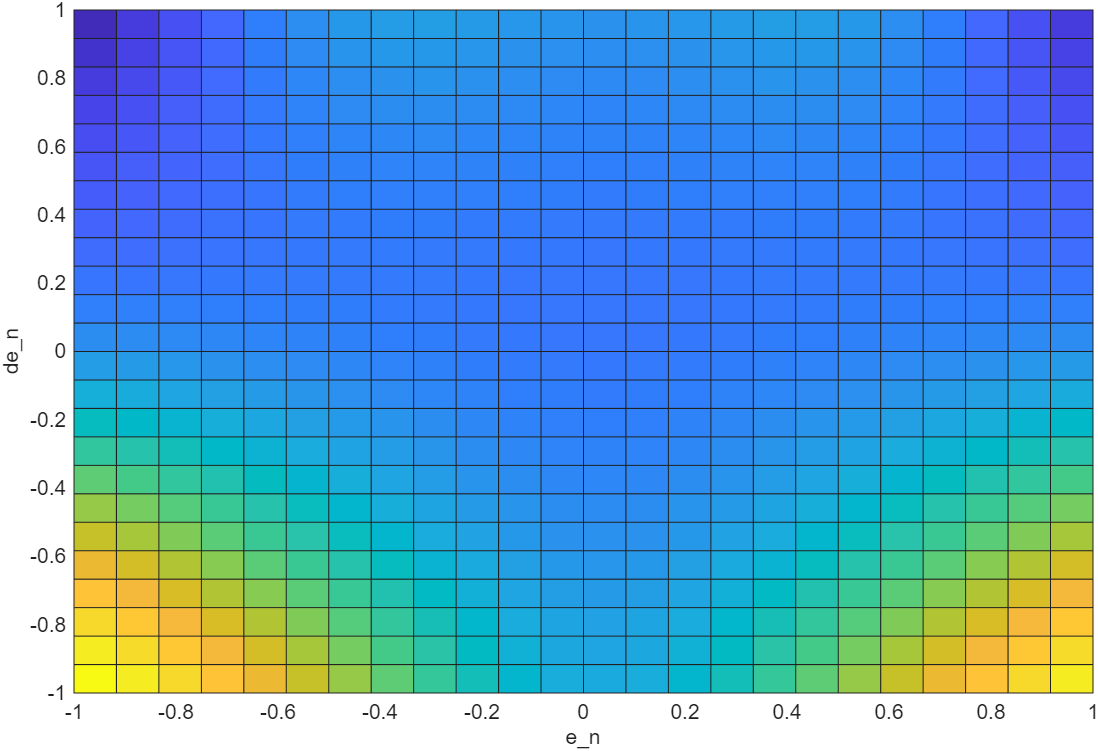
\includegraphics[width=0.45\textwidth]{img/fuzzy_alpha_p}}
		\hspace{2mm}
		\subfloat[سطح کنترلی تنظیم‌کننده انتگرالی ($\alpha_i$)]{
			\label{fig:method-surface-alphai}
			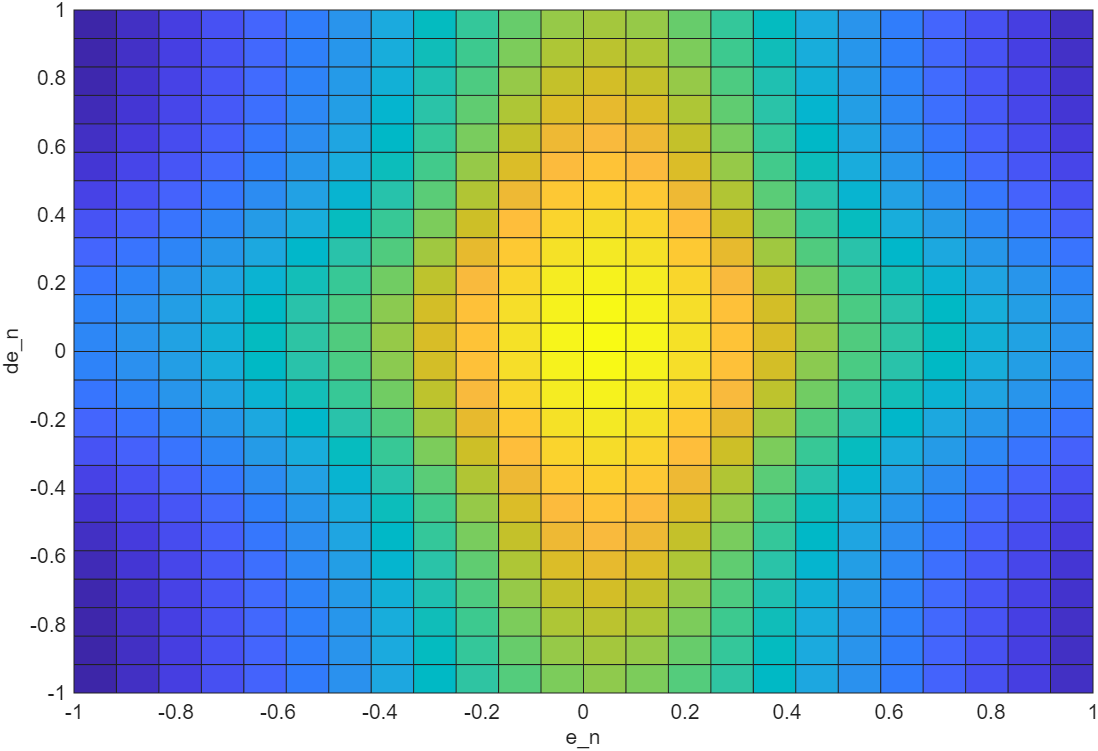
\includegraphics[width=0.45\textwidth]{img/fuzzy_alpha_i}}
		\\
		\subfloat[سطح کنترلی تنظیم‌کننده مشتقی ($\alpha_d$)]{
			\label{fig:method-surface-alphad}
			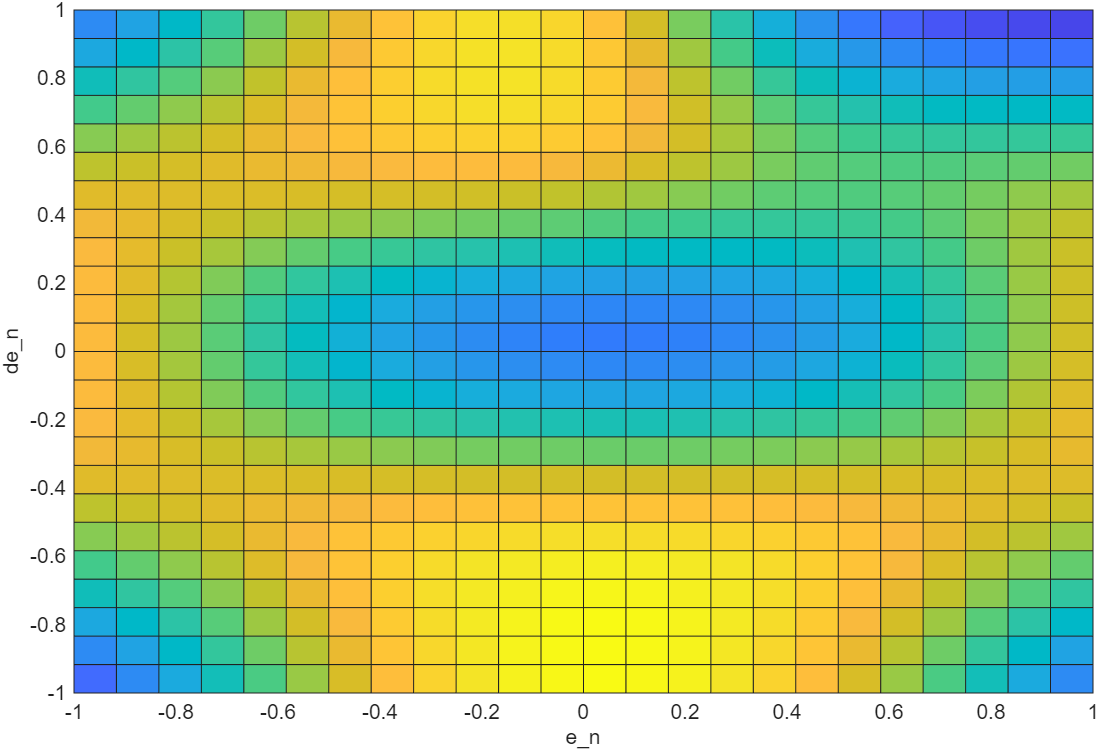
\includegraphics[width=0.45\textwidth]{img/fuzzy_alpha_d}}
		\caption{سطوح کنترلی سیستم استنتاج فازی؛ نشان‌دهنده تغییرات خروجی‌ها نسبت به فضای خطای ورودی}
		\label{fig:method-fuzzy-surfaces}
	\end{figure}
	
	\paragraph{غیرفازی‌سازی و مقیاس‌بندی خروجی (\lr{Defuzzification and Gain Scaling})}
	گام نهایی در هسته فازی، استخراج یک مقدار قطعی عددی از درجات تحقق قوانین است که به آن غیرفازی‌سازی می‌گویند. با توجه به استفاده از خروجی‌های سینگلتون، روش کارآمد میانگین وزن‌دار (\lr{Weighted Average}) برای این منظور به کار رفته است. مقدار نهایی هر خروجی ($\alpha_x$) طبق معادله (\ref{eq:method-defuzzification}) به دست می‌آید:
	
	\begin{equation} \label{eq:method-defuzzification}
		\alpha_x = \frac{\sum_{k=1}^{N} f_k \cdot w_k}{\sum_{k=1}^{N} f_k} \quad , \quad x \in \{p, i, d\}
	\end{equation}
	
	که در آن $N=25$ تعداد کل قوانین، $f_k$ درجه تحقق محاسبه شده برای هر قانون، و $w_k$ مقادیر عددی خروجی‌های تک‌مقداری (سینگلتون) متناظر با متغیرهای زبانی است که جزئیات آن‌ها در جدول \ref{tab:method-output-mfs} ذکر شده است.
	
	\begin{table}[htbp]
		\centering
		\caption{مقادیر عددی سینگلتون برای مجموعه‌های فازی خروجی}
		\label{tab:method-output-mfs}
		\begin{tabular}{|c|c|c|}
			\hline
			\textbf{توصیف‌گر زبانی خروجی} & \textbf{نماد} & \textbf{مقدار خروجی ($w_k$)} \\
			\hline
			بسیار کم & \lr{VL} & $0$ \\
			کم & \lr{L} & $0.25$ \\
			متوسط & \lr{M} & $0.5$ \\
			زیاد & \lr{H} & $0.75$ \\
			بسیار زیاد & \lr{VH} & $1$ \\
			\hline
		\end{tabular}
	\end{table}
	
	خروجی‌های مستقیم سیستم فازی ($\alpha_p, \alpha_i, \alpha_d$) صرفاً مقادیری بدون بعد در بازه $[0, 1]$ هستند. برای اینکه این مقادیر بتوانند نقش ضرایب فیزیکی کنترل‌کننده ($K_p, K_i, K_d$) را ایفا کنند، از یک نگاشت خطی بهره گرفته می‌شود:
	
	\begin{align}
		K_p &= K_{p,min} + (K_{p,max} - K_{p,min}) \times \alpha_p \\
		K_i &= K_{i,min} + (K_{i,max} - K_{i,min}) \times \alpha_i \\
		K_d &= K_{d,min} + (K_{d,max} - K_{d,min}) \times \alpha_d
		\label{eq:method-gain-mapping}
	\end{align}
	
	در پیاده‌سازی عملی این معماری، این عملگرهای نگاشت از طریق اعمال ضرایب مقیاس‌بندی خروجی ($G_P, G_I, G_D$) بر خروجی‌های خام فازی انجام می‌پذیرد. مقادیر این ضرایب به همراه ضرایب نرمال‌سازی ورودی ($G_E$) به دلیل تفاوت در دینامیک محورهای مختلف، برای هر یک از درجات آزادی انتقالی و دورانی به صورت مجزا تنظیم شده‌اند. فرآیند کالیبراسیون این ضرایب از طریق سعی و خطا در محیط شبیه‌ساز صورت گرفته و مقادیر نهایی و بهینه‌شده در جدول \ref{tab:method-fuzzy-gains} گزارش گردیده‌اند.
	
\begin{table}[htbp]
	\centering
	\small  % or \footnotesize if still too wide
	\caption{ضرایب نهایی پیش‌پردازش ورودی و مقیاس‌بندی خروجی‌ها برای کنترل‌کننده‌های فازی در درجات آزادی مختلف}
	\label{tab:method-fuzzy-gains}
	\begin{tabular}{|c|c|c|c|c|}
		\hline
		\textbf{محور} & \textbf{$G_E$ (خطا)} & \textbf{$G_P$ (تناسبی)} & \textbf{$G_I$ (انتگرالی)} & \textbf{$G_D$ (مشتقی)} \\ \hline \hline
		انتقالی افقی (\lr{x, y}) & $16.6$ & $0.5$ & $0.03$ & $6$ \\ \hline
		انتقالی عمودی (\lr{z}) & $20$ & $50$ & $50$ & $10$ \\ \hline
		دورانی ($\alpha, \beta, \gamma$) & $0.25$ & $0.5$ & $0.03$ & $6$ \\ \hline
	\end{tabular}
\end{table}
	
	\subsection{ملاحظات پایداری و مدل‌سازی در سیمولینک}
	\label{subsec:method-simulink}
	برای پیاده‌سازی نهایی این منطق در نرم‌افزار \lr{MATLAB/Simulink} و اتصال آن به شبیه‌ساز از طریق گره‌های \lr{ROS}، ملاحظات زیر در طراحی مدل سیمولینک لحاظ گردید:
	
	\begin{enumerate}
		\item \textbf{فیلتر مشتق‌گیر نویز:} به دلیل ماهیت گسسته شبیه‌سازی در \lr{Gazebo}، محاسبه مستقیم مشتق خطا ($de_n$) می‌تواند منجر به تولید نویزهای فرکانس بالا و ناپایداری در سیگنال کنترلی شود. برای رفع این مشکل، یک فیلتر پایین‌گذر با ضریب فیلتر $N=10$ در بلوک مشتق‌گیر تعبیه شد تا ضمن حفظ فاز سیگنال، از اسپایک‌های (\lr{Spikes}) عددی جلوگیری کند.
		
		\item \textbf{جبران‌ساز پیش‌خور گرانش (\lr{Gravity Feed-forward}):} یکی از چالش‌های اساسی در کنترل محور $Z$، غلبه بر وزن ربات بود. با توجه به اینکه جرم مدل شبیه‌سازی‌شده معادل ۶.۶ کیلوگرم است، نیروی گرانشی در حدود ۶۸ نیوتن همواره به سیستم رو به پایین وارد می‌شود. برای جلوگیری از اشباع (\lr{Windup}) انتگرال‌گیرِ کنترلر و بهبود سرعت پاسخ، یک مقدار ثابت معادل $68\text{ N}$ به عنوان سیگنال پیش‌خور مستقیماً به خروجی نهایی کنترل‌کننده محور ارتفاع ($Z$) اضافه گردید. این طراحی باعث می‌شود \lr{Fuzzy PID} تنها مسئولیت خنثی‌سازی خطاهای دینامیکی و اینرسی را بر عهده داشته باشد.
	\end{enumerate}
	
	\subsection{مدیریت گذار حالت و منطق کنترلی دو فازی (\lr{Two-Phase Control Logic})}
	\label{subsec:method-state-machine}
	
	یکی از چالش‌های اساسی در کنترل ربات‌های معلق یا سیستم‌هایی که با سطح در تماس فیزیکی هستند، تداخل نیروهای تماسی (اصطکاک و برخورد) با منطق کنترل‌کننده است. مادامی که بخش متحرک دستگاه روی سطح زمین قرار دارد، فعال بودن کنترل‌کننده‌های وضعیت منجر به تولید فرامین نامعتبر، اشباع انتگرال‌گیرها (\lr{Integrator Windup}) و ناپایداری به دلیل مقاومت فیزیکی سطح می‌شود. برای حل این مشکل، یک معماری کنترلی دو فازی مبتنی بر ماشین حالت (\lr{State Machine}) در محیط \lr{Simulink/Stateflow} طراحی و پیاده‌سازی گردید که عملکرد سیستم را به دو حالت مجزای «مستقر روی زمین» (\lr{OnGround}) و «معلق» (\lr{Levitating}) تقسیم می‌کند.
	
	\subsubsection{ساختار ماشین حالت و تشخیص فاز}
	\label{subsubsec:method-state-machine-structure}
	برای تشخیص فاز کاری سیستم، از داده‌های موقعیت محور عمودی ($z_{meas}$) و سرعت خطی آن ($dz_{meas}$) استفاده می‌شود. همان‌طور که در معماری مدل مشخص است، سرعت عمودی از طریق اعمال یک فیلتر مشتق‌گیر زمان‌گسسته با تابع تبدیل $\frac{K(z-1)}{T_s z}$ بر روی سیگنال موقعیت محاسبه می‌گردد. ماشین حالت طراحی‌شده دارای دو وضعیت اصلی و شروط گذار (\lr{Transition Conditions}) به شرح زیر است:
	
	\begin{enumerate}
		\item \textbf{وضعیت مستقر روی زمین (\lr{OnGround}):} 
		در این حالت، سیگنال فعال‌ساز کنترل‌کننده قطع است (\lr{enable = 0}). سیستم در این وضعیت باقی می‌ماند تا زمانی که شرایط برخاستن به صورت پایدار ارضا شود. شرط گذار به حالت معلق این است که ارتفاع دستگاه از یک آستانه مشخص فراتر رود ($z_{meas} \geq z_{on}$) و همزمان نوسانات سرعتی آن محدود باشد ($|dz_{meas}| \leq dz_{tol}$). برای اطمینان از پایداری این گذار و جلوگیری از سوئیچینگ بر اثر نویز، این شرایط باید برای تعداد مشخصی از گام‌های زمانی متوالی ($N_{on}$) برقرار بماند.
		
		\item \textbf{وضعیت معلق (\lr{Levitating}):}
		با ورود به این فاز، فرمان فعال‌سازی صادر می‌شود (\lr{enable = 1}). بازگشت به حالت روی زمین تنها در صورتی رخ می‌دهد که ارتفاع ربات برای تعداد $N_{off}$ گام زمانی متوالی، کمتر از آستانه نشستن ($z_{off}$) ارزیابی شود.
	\end{enumerate}
	
	\subsubsection{منطق سوئیچینگ و ریست کنترل‌کننده‌ها (\lr{Reset Logic})}
	\label{subsubsec:method-reset-logic}
	خروجی سیگنال \lr{enable} از ماشین حالت (که در مدل با عنوان \lr{Phase Switch Enable} شناخته می‌شود)، وارد مجموعه‌ای از بلوک‌های سوئیچ می‌گردد. اگر مقدار این سیگنال بزرگتر از $0.5$ باشد، فرامین کنترلی محاسبه‌شده ($F_x, F_y, T_x, T_y, T_z$) به عملگرها ارسال می‌شوند و در غیر این صورت، مقدار صفر به خروجی تخصیص می‌یابد تا از اعمال هرگونه نیروی ناخواسته در زمان استقرار روی زمین جلوگیری شود.
	
	یک الزام حیاتی در این معماری، مدیریت حافظه داخلی کنترل‌کننده‌ها (مقادیر پیشین در انتگرال‌گیر و مشتق‌گیر) در لحظه فعال‌سازی است. اگر کنترل‌کننده‌ها صرفاً فعال شوند اما داده‌های حافظه آن‌ها پاک نشود، محاسبه خطا بر اساس داده‌های قدیمی (مربوط به زمان استقرار) منجر به تولید یک فرمان کنترلی بسیار بزرگ (\lr{Control Spike}) در لحظه اول می‌شود که ناپایداری شدید و پرش ربات را به همراه خواهد داشت. 
	
	برای رفع این مشکل، ماشین حالت به گونه‌ای طراحی شده است که دقیقاً در بلوک \lr{entry} وضعیت \lr{Levitating}، سیگنال ریست را فعال می‌کند (\lr{reset = 1}). سپس در بلوک \lr{during}، با استفاده از منطق \lr{after(1, tick)}، این سیگنال بلافاصله در گام شبیه‌سازی بعدی غیرفعال می‌شود (\lr{reset = 0}). این پالسِ تک‌گامی به بلوک‌های کنترلی ارسال شده و تضمین می‌کند که تمامی حافظه‌های خطا پیش از آغاز به کار در فاز معلق پاک‌سازی شده و سیستم، کنترل خود را با خطای صفرِ اولیه و به صورت کاملاً نرم (\lr{Smooth Transfer}) آغاز نماید.\autoref{fig:method-state-machine}
	
	\begin{figure}[htbp]
		\centering
		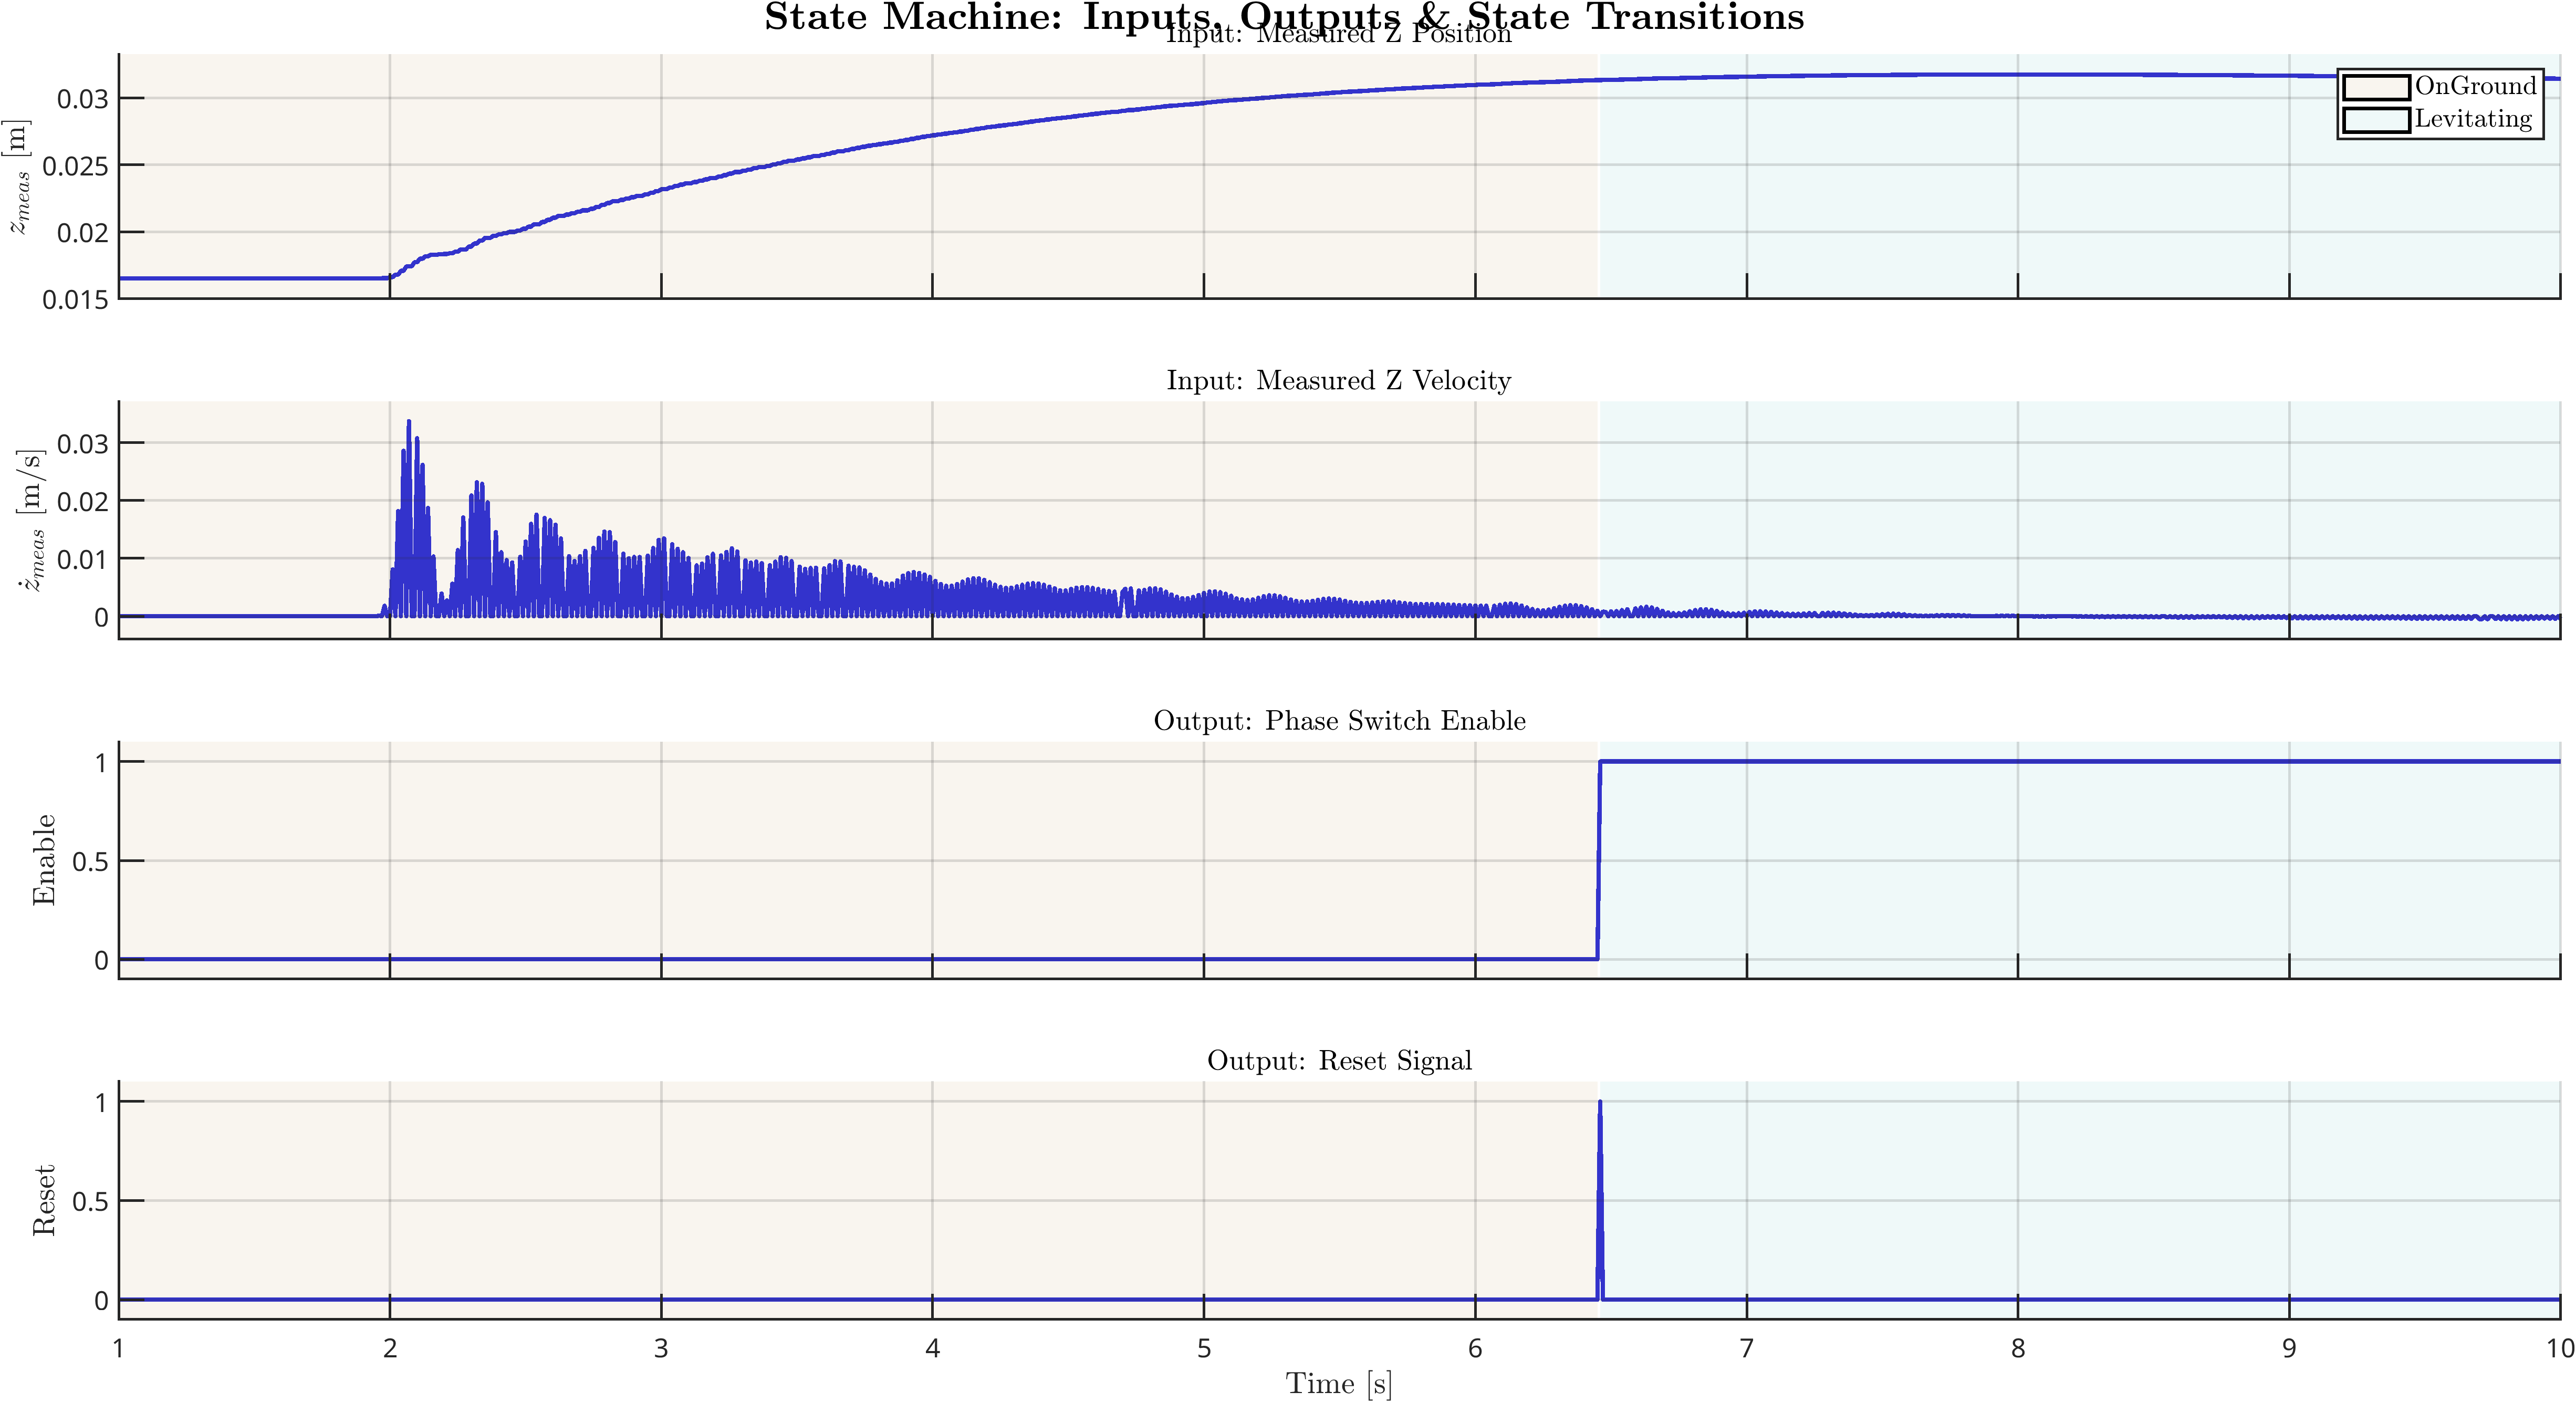
\includegraphics[width=0.7\linewidth]{Results/State_Machine/state-machine}
		\caption{ساختار ماشین حالت کنترل دو مرحله ای}
		\label{fig:method-state-machine}
	\end{figure}
	
	
	\subsubsection{فیلتر داده‌های نامعتبر (\lr{NaN Filter}) و ایمن‌سازی ارتباطات}
	\label{subsubsec:method-nan-filter}
	
	یکی از چالش‌های رایج در پیاده‌سازی سیستم‌های نرم‌افزار در حلقه (\lr{Software-in-the-Loop}) و برقراری ارتباط بین محیط شبیه‌ساز (مانند \lr{Gazebo}) و کنترل‌کننده در \lr{Simulink}، ناپایداری‌های گذرا در لحظات اولیه راه‌اندازی است. در کسری از ثانیه در ابتدای اجرای شبیه‌ساز، به دلیل تأخیر در مقداردهی اولیه سنسورها، عدم همگام‌سازی کامل گره‌های ارتباطی یا از دست رفتن بسته‌های داده در شبکه، احتمال دریافت داده‌های مفقود یا نامعتبر وجود دارد. این داده‌های نامعتبر در محیط \lr{Simulink} به صورت \lr{NaN} (\lr{Not-a-Number}) تفسیر می‌شوند.
	
	ورود مقادیر \lr{NaN} به معماری کنترلی، به ویژه در بلوک‌های دارای حافظه داخلی مانند انتگرال‌گیرها یا مشتق‌گیرها، باعث انتشار دائمی خطا در کل حلقه کنترل می‌شود. در این حالت، فرمان‌های نیرو و گشتاور ارسالی به شبیه‌ساز نیز نامعتبر شده و منجر به فروپاشی فیزیکی شبیه‌سازی یا رفتار کاملاً غیرقابل پیش‌بینی ربات می‌گردد.
	
	برای جلوگیری از این پدیده، یک مکانیزم محافظتی تحت عنوان فیلتر داده‌های نامعتبر (\lr{NaN Filter}) بلافاصله پس از محاسبه سیگنال خطا (تفاضل مقادیر سنسور و مقادیر مطلوب) تعبیه شده است. همان‌طور که در مدل مشخص است، سیگنال خطا پیش از ورود به مسیر اصلی، توسط تابع \lr{isnan} ارزیابی می‌شود. خروجی منطقی این بلوک، وضعیت یک بلوک سوئیچ (\lr{Switch}) را تعیین می‌کند:
	
	\begin{itemize}
		\item \textbf{در صورت دریافت داده نامعتبر:} اگر شرط $\mathrm{isnan} > 0.5$ برقرار باشد (یعنی حداقل یکی از درایه‌های بردار خطا \lr{NaN} باشد)، سوئیچ مسیر داده‌های ورودی را قطع کرده و یک بردار خطای پیش‌فرض و ایمن (در این پیاده‌سازی بردار $[0, 0, 0, 0.04, 0, 0.2]$) را به عنوان سیگنال جایگزین به کنترل‌کننده‌ها تزریق می‌کند. این مقادیر اولیه تضمین می‌کنند که کنترل‌کننده در لحظه شروع به کارِ شبیه‌ساز، واکنش شدید و ناگهانی نشان ندهد.
		\item \textbf{در شرایط کارکرد عادی:} به محض پایداری ارتباط و دریافت داده‌های عددی معتبر از شبیه‌ساز، شرط سوئیچ نقض شده و بلوک، سیگنال خطای واقعی سیستم را به سمت بخش نرمال‌سازی و هسته فازی عبور می‌دهد.
	\end{itemize}
	
	
	این منطق سوئیچینگ ساده اما حیاتی، تضمین می‌کند که راه‌اندازی سیستم همواره با مقادیر معین و پایدار صورت پذیرفته و پایداری عددی شبیه‌ساز در برابر خطاهای ارتباطی حفظ شود.
	
	\section[ماژول تولید و برنامه‌ریزی مسیر]{ماژول تولید و برنامه‌ریزی مسیر\footnote{Trajectory Generation}}
	\label{sec:method-trajectory}
	
	یکی از چالش‌های اساسی در کنترل ربات‌ها، جلوگیری از اعمال فرامین ناگهانی و تغییرات پله‌ای به سیستم کنترلی است. تغییرات ناگهانی در نقاط مرجع\footnote{Reference Setpoints} می‌تواند منجر به اشباع عملگرها، نوسانات شدید و در نهایت ناپایداری سیستم شود. برای رفع این مشکل، ماژول تولید مسیر وظیفه دارد تا فرامین موقعیت و جهت‌گیری دریافت شده از شبیه‌ساز (محیط \lr{ROS}) را به مسیرهای پیوسته و هموار تبدیل کند. بدین منظور، ساختار این بخش به دو زیرسیستم مجزا تقسیم شده است: «رمزگشای فرمان»\footnote{Command Decoder} و «برنامه‌ریز مسیر»\footnote{Trajectory Planner}. این معماری برای هر دو کانال موقعیت\footnote{Position} و جهت‌گیری
	\footnote{Orientation} به صورت مشابه پیاده‌سازی شده است.
	
	\subsection{رمزگشای فرمان}
	\label{subsec:method-command-decoder}
	بلوک رمزگشای فرمان به عنوان رابط اولیه میان پیام‌های دریافتی از شبکه \lr{ROS} و سیستم برنامه‌ریز مسیر عمل می‌کند. وظیفه اصلی این بلوک، دریافت داده‌های هدف (شامل موقعیت یا جهت‌گیری، زمان تخصیص‌یافته برای حرکت و شناسه توالی پیام) و استخراج یک فرمان معتبر برای شروع یک حرکت جدید است. 
	
	در طراحی این بلوک، ملاحظات ایمنی و پایداری زیر در نظر گرفته شده است:
	\begin{itemize}
		\item \textbf{تشخیص فرامین جدید مبتنی بر شناسه توالی\footnote{Sequence ID}:} سیستم به طور پیوسته متغیر شناسه توالی ($seq$) را بررسی می‌کند. فرمان جدید تنها زمانی به برنامه‌ریز صادر می‌شود (تغییر پرچم $start\_new = 1.0$) که شناسه پیام دریافتی با شناسه ذخیره شده از پیام قبلی ($last\_seq$) تفاوت داشته باشد. این امر از اجرای مجدد و مکرر یک مسیر تکراری جلوگیری می‌کند.
		\item \textbf{مقداردهی اولیه ایمن\footnote{Robust Initialization}:} به جای فرض مقادیر صفر، سیستم با استفاده از متغیرهای ماندگار\footnote{Persistent} از مقادیر واقعی راه‌اندازی می‌شود. به عنوان مثال، در ماژول موقعیت، نقطه اولیه به فرمت سه بعدی $[0; 0; 16.6]$ و در ماژول جهت‌گیری (\lr{Roll, Pitch, Yaw}) با مقادیر $[0; 0; 0.2]$ مقداردهی اولیه می‌شود.
		\item \textbf{اعتبارسنجی ابعاد و مقادیر\footnote{Sanity Checks}:} تابع کمکی \lr{\texttt{force3}} اطمینان حاصل می‌کند که بردار ورودی همواره یک بردار ستونی سه‌بعدی است. همچنین، زمان اجرای حرکت ($duration$) برای جلوگیری از تقسیم بر صفر یا تولید سرعت‌های بی‌نهایت، به یک مقدار حداقل محدود شده است (مانند $10^{-3}$ ثانیه).
	\end{itemize}
	
	\subsection[برنامه‌ریز مسیر مبتنی بر چندجمله‌ای مرتبه پنج]{برنامه‌ریز مسیر مبتنی بر چندجمله‌ای مرتبه پنج\footnote{Quintic Trajectory Planner}}
	\label{subsec:method-quintic-planner}
	
	پس از تایید و ارسال فرمان جدید از سوی رمزگشا، بلوک برنامه‌ریز مسیر وظیفه تولید نقاط مرجع زمان‌پیوسته را بر عهده دارد. برای تضمین پیوستگی در موقعیت (یا زاویه)، سرعت و شتاب، از چندجمله‌ای‌های مرتبه پنج\footnote{Quintic Polynomials} استفاده شده است. معادله مسیر برای هر یک از درایه‌های سه‌بعدی به فرمت زیر تعریف می‌شود:
	$$ p(\tau) = c_0 + c_1 \tau + c_2 \tau^2 + c_3 \tau^3 + c_4 \tau^4 + c_5 \tau^5 $$
	که در آن $\tau$ زمان محلی\footnote{Local Time} سپری شده از ابتدای حرکت جدید است ($0 \le \tau \le T_{seg}$). با مشتق‌گیری از رابطه فوق، پروفایل‌های سرعت و شتاب مرجع نیز به صورت زیر به دست می‌آیند:
	$$ v(\tau) = c_1 + 2c_2 \tau + 3c_3 \tau^2 + 4c_4 \tau^3 + 5c_5 \tau^4 $$
	$$ a(\tau) = 2c_2 + 6c_3 \tau + 12c_4 \tau^2 + 20c_5 \tau^3 $$
	
	برای محاسبه ضرایب $c_i$ در هر راستا، سیستم از شرایط مرزی در لحظه شروع حرکت ($\tau = 0$) و پایان حرکت ($\tau = T_{seg}$) استفاده می‌کند. حالت اولیه ($p_0, v_0, a_0$) از آخرین وضعیت ذخیره شده در حافظه داخلی سیستم\footnote{Latching State} استخراج می‌شود تا هیچ‌گونه پرشی در نقطه اتصال دو مسیر ایجاد نشود. شرایط انتهایی ($p_1, v_1, a_1$) نیز شامل نقطه هدف نهایی با فرض سرعت و شتاب نهایی صفر ($v_1=0$ و $a_1=0$) تنظیم می‌گردند. این شرایط منجر به تشکیل یک دستگاه معادلات خطی به فرم $A \mathbf{c} = \mathbf{b}$ می‌شود:
	$$
	\begin{bmatrix}
		1 & 0 & 0 & 0 & 0 & 0 \\
		0 & 1 & 0 & 0 & 0 & 0 \\
		0 & 0 & 2 & 0 & 0 & 0 \\
		1 & T & T^2 & T^3 & T^4 & T^5 \\
		0 & 1 & 2T & 3T^2 & 4T^3 & 5T^4 \\
		0 & 0 & 2 & 6T & 12T^2 & 20T^3
	\end{bmatrix}
	\begin{bmatrix}
		c_0 \\ c_1 \\ c_2 \\ c_3 \\ c_4 \\ c_5
	\end{bmatrix}
	=
	\begin{bmatrix}
		p_0 \\ v_0 \\ a_0 \\ p_1 \\ 0 \\ 0
	\end{bmatrix}
	$$
	سیستم با حل این ماتریس، مقادیر $c_0$ تا $c_5$ را محاسبه کرده و پروفایل مسیر را ارزیابی می‌کند. در صورتی که زمان محلی از زمان کل تخصیص‌یافته فراتر رود ($\tau \ge T_{seg}$)، پرچم اتمام حرکت ($done = 1.0$) فعال شده و وضعیت نهایی به عنوان نقطه شروع حرکت‌های آتی حفظ می‌شود. در این حالت (رفتار غیرفعال\footnote{Inactive Behavior})، سرعت و شتاب‌های مرجع خروجی دقیقاً برابر صفر قرار می‌گیرند.
	
	\begin{figure}[htbp]
		\centering
		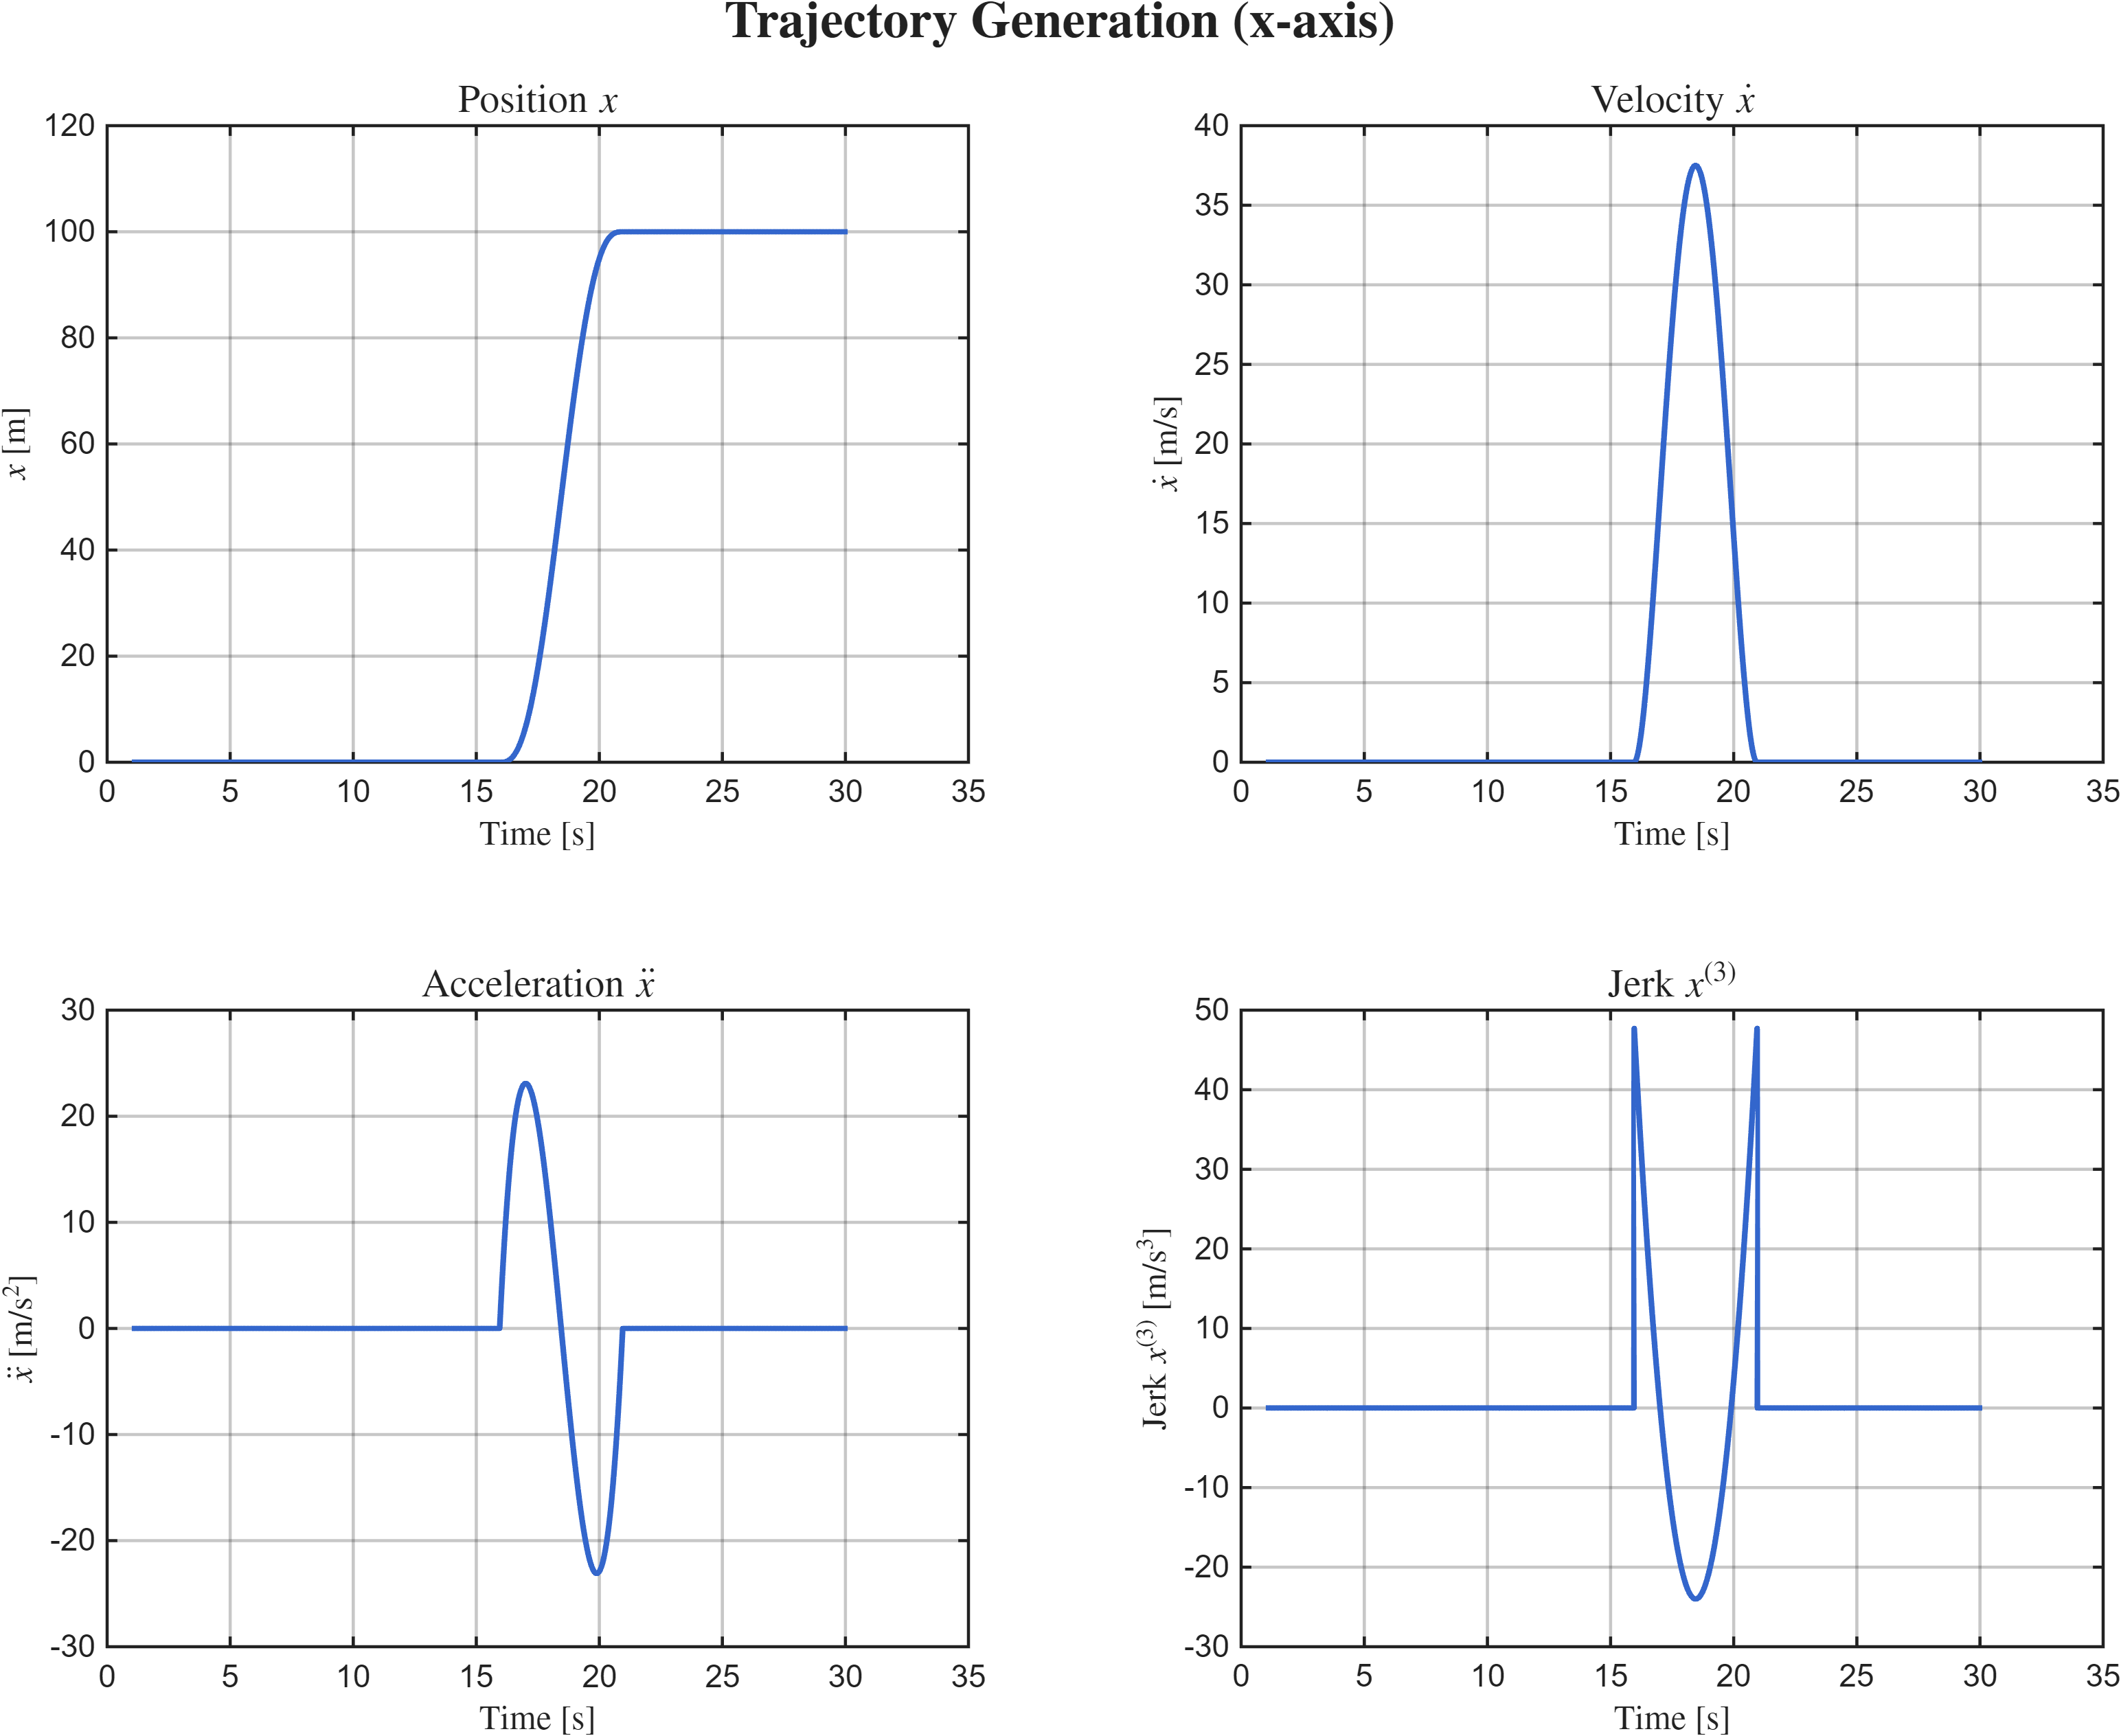
\includegraphics[width=0.7\linewidth]{img/trajectory_generation_x}
		\caption{نمونه مسیر درجه 5}
		\label{fig:method-quintic-example}
	\end{figure}
	
	
	
	\subsection[ملاحظات طراحی برای جهت‌گیری]{ملاحظات طراحی برای جهت‌گیری\footnote{Orientation Specifics}}
	\label{subsec:method-orientation-specifics}
	
	منطق برنامه‌ریزی برای زوایای اویلر (\lr{Roll, Pitch, Yaw}) کاملاً مشابه مسیر موقعیت است؛ با این حال، به دلیل ماهیت دایره‌ای زوایا، یک چالش اساسی در دوران حول محور عمودی (زاویه \lr{Yaw}) وجود دارد. اگر ربات نیاز به تغییر زاویه از $170^\circ$ به $-170^\circ$ داشته باشد، محاسبه تفاضل ساده منجر به تولید فرمانی برای دوران $340^\circ$ درجه در خلاف جهت مطلوب می‌شود که از نظر سینماتیکی نامطلوب است.
	
	برای حل این مشکل، در ماژول \lr{\texttt{traj\_planner\_orientation}} از مکانیزم همپوشانی فاز\footnote{Phase Wrapping} برای یافتن کوتاه‌ترین مسیر دورانی استفاده شده است. این عملیات توسط تابع ریاضی زیر پیاده‌سازی می‌گردد:
	$$ \Delta \text{yaw} = \text{atan2}(\sin(\psi_1 - \psi_0), \cos(\psi_1 - \psi_0)) $$
	که در کد با عنوان تابع کمکی \lr{\texttt{wrapToPi}} تعبیه شده است. با استفاده از این تکنیک، اختلاف زاویه هدف و زاویه فعلی همواره به بازه $[-\pi, \pi]$ محدود می‌شود و زاویه هدف جدید ($\psi_1$) بر اساس این تفاضل مینیمم تصحیح می‌گردد. در نهایت، سیگنال‌های مرجع پیوسته تولید شده شامل موقعیت، سرعت و شتاب خطی و زاویه‌ای، برای مقایسه با مقادیر اندازه‌گیری شده از سنسورها (فیدبک) به بلوک مقایسه‌گر\footnote{Comparator} و سپس به کنترلر ارسال می‌شوند.
	
\section{تحلیل تکینگی سینماتیکی و ارزیابی مهارت فضای کار}
\label{sec:method-singularity}

در این بخش، به بررسی رفتار سینماتیکی مکانیزم و شناسایی پیکربندی‌های تکین (\lr{Singularity Configurations}) پرداخته می‌شود. هسته اصلی این تحلیل، ماتریس انتقال $\Gamma$ (ماتریس ژاکوبین شبه‌استاتیکی) است که ارتباط‌دهنده فضای جریان‌های سیم‌پیچ‌ها (ورودی عملگرها) به فضای پیچش (\lr{Wrench}) نیرو و گشتاور اعمال‌شده بر متحرک (خروجی مجری نهایی) می‌باشد. با توجه به پیچیدگی معادلات سینماتیکی و ابعاد بالای پیکربندی سیستم، استخراج تحلیلی کامل نقاط تکین امکان‌پذیر نیست؛ از این رو، از یک رویکرد ترکیبی شامل تحلیل تحلیلی مبتنی بر معادلات میدان مغناطیسی و نیز شبیه‌سازی عددی مبتنی بر جستجوی شبکه‌ای (\lr{Grid-Search}) استفاده شده است.

\subsection{بازنمایی ریاضی ماتریس $\Gamma$}
\label{subsec:method-gamma-definition}

همان‌طور که در روابط پیشین (بخش \ref{subsec:method-stator-model}) بیان شد، ماتریس $\Gamma$ به ابعاد $6 \times n$ (که $n$ تعداد سیم‌پیچ‌های فعال است، در اینجا $n=16$) برای یک وضعیت مشخص از متحرک (موقعیت و جهت) به صورت زیر تعریف می‌گردد:

\[
\Gamma(\mathbf{q}) = 
\begin{bmatrix}
	\frac{\partial \mathbf{F}}{\partial I_1} & \frac{\partial \mathbf{F}}{\partial I_2} & \cdots & \frac{\partial \mathbf{F}}{\partial I_n} \\[4pt]
	\frac{\partial \mathbf{T}}{\partial I_1} & \frac{\partial \mathbf{T}}{\partial I_2} & \cdots & \frac{\partial \mathbf{T}}{\partial I_n}
\end{bmatrix}
=
\begin{bmatrix}
	\mathbf{w}_1 & \mathbf{w}_2 & \cdots & \mathbf{w}_n
\end{bmatrix}
\]

که در آن $\mathbf{q} = (x,y,z,\alpha,\beta,\gamma)$ بردار مختصات تعمیم‌یافته متحرک است، $\mathbf{F} = [F_x,F_y,F_z]^T$ نیروی کل وارد بر متحرک، $\mathbf{T} = [T_x,T_y,T_z]^T$ گشتاور کل، و $I_j$ جریان الکتریکی سیم‌پیچ $j$-ام می‌باشد. ستون $j$-ام ماتریس $\Gamma$ یعنی $\mathbf{w}_j$، بردار پیچش حاصل از واحد جریان در سیم‌پیچ $j$-ام است.

رابطه بین پیچش مطلوب $\mathbf{W}_{des} = [\mathbf{F}^T, \mathbf{T}^T]^T$ و جریان‌های سیم‌پیچ‌ها به صورت خطی زیر نوشته می‌شود:

\[
\mathbf{W}_{des} = \Gamma(\mathbf{q}) \, \mathbf{I}
\]
\label{eq:method-wrench-des}
که در آن $\mathbf{I} = [I_1,I_2,\dots,I_n]^T$ بردار جریان‌ها است.

\subsection{تجزیه مقادیر تکین (\lr{Singular Value Decomposition})}
\label{subsec:method-svd-analysis}

برای تحلیل کیفی و کمی ماتریس $\Gamma$ در هر پیکربندی، از روش تجزیه مقادیر تکین (SVD) استفاده می‌شود. بر اساس قضیه SVD، هر ماتریس حقیقی $\Gamma$ با ابعاد $m \times n$ (در اینجا $m=6$ و $n=16$) را می‌توان به صورت حاصل‌ضرب سه ماتریس نوشت:

\[
\Gamma = U \, \Sigma \, V^T
\]
\label{eq:method-svd-gamma}
که در آن $U$ و $V$ ماتریس‌های متعامد و $\Sigma$ ماتریسی قطری شامل مقادیر تکین $\sigma_1 \ge \sigma_2 \ge \dots \ge \sigma_m \ge 0$ است.

\subsection{عدد شرط به عنوان معیار اصلی}
\label{subsec:method-condition-number}

عدد شرط ماتریس $\Gamma$ به صورت نسبت بزرگ‌ترین مقدار تکین به کوچک‌ترین مقدار تکین تعریف می‌شود:
\[
\kappa(\Gamma) = \frac{\sigma_{\max}}{\sigma_{\min}}
\]
\label{eq:method-condition-number}

در حالت ایده‌آل (ایزوتروپیک کامل)، $\kappa = 1$ است. با نزدیک شدن سیستم به یک پیکربندی تکین، $\sigma_{\min} \to 0$ و در نتیجه $\kappa \to \infty$ می‌رود. هر چه $\kappa$ بزرگتر باشد، ماتریس بدشرط‌تر (\lr{Ill-conditioned}) بوده و محاسبه وارون شبه‌مور-پنروز با ناپایداری عددی همراه خواهد شد. در شبیه‌سازی، مقادیر بسیار بزرگ $\kappa$ منجر به واگرایی عددی و خروج از حالت پایدار می‌شوند. در این پژوهش، به دلیل سادگی تفسیر، تمرکز اصلی بر عدد شرط خواهد بود و معیارهای دیگر (نظیر حاصل‌ضرب مقادیر تکین) استفاده نمی‌شوند.

در محاسبات عددی، به دلیل خطاهای گرد کردن، مقادیر تکین بسیار کوچک (کوچک‌تر از آستانه $\epsilon = 10^{-12}$) عملاً صفر در نظر گرفته می‌شوند. اگر تمام مقادیر تکین از $\epsilon$ کوچک‌تر باشند، سیستم در حالت تکین کامل قرار داشته و $\kappa = \infty$ در نظر گرفته می‌شود.

\subsection{تکینگی‌های ذاتی ناشی از ساختار میدان مغناطیسی و مدل تحلیلی}
\label{subsec:method-singularity-analysis}

بررسی معادلات نیرو و گشتاور استخراج‌شده (روابط \ref{eq:method-force-components} تا \ref{eq:method-torque-components}) نشان می‌دهد که وابستگی به زاویه $\gamma$ به صورت ضمنی از طریق ماتریس دوران $R$ و مؤلفه‌های $c^m_1$ و $c^m_2$ ظاهر می‌شود. دو نوع تکینگی مستقیماً از این ساختار ریاضی ناشی می‌شوند که هر یک ماهیت متفاوتی دارند اما هر دو در مجاورت زوایای خاصی از $\gamma$ خود را نشان می‌دهند.

\subsubsection{تکینگی فیزیکی در $\gamma = \pm\pi$ (و مضارب آن)}

در پیکربندی‌ای که $\gamma = \pm\pi$ (یعنی متحرک ۱۸۰ درجه چرخیده)، بردارهای میدان مغناطیسی آرایه هالباخ نسبت به سیم‌پیچ‌های ثابت کاملاً متقارن می‌شوند. برای اثبات این پدیده، فرض کنید $\alpha = \beta = 0$ و متحرک در مکان $(x_m, y_m)$ قرار دارد. ماتریس دوران در این حالت به
\[
R(\gamma) = \begin{bmatrix}
	\cos\gamma & \sin\gamma & 0 \\
	-\sin\gamma & \cos\gamma & 0 \\
	0 & 0 & 1
\end{bmatrix}
\]
تبدیل می‌شود. در نتیجه، مولفه‌های بردار $\mathbf{c}^m$ به صورت زیر خواهند بود:
\[
c_1^m(\gamma) = \cos\gamma\,(x_c - x_m) + \sin\gamma\,(y_c - y_m),\qquad
c_2^m(\gamma) = -\sin\gamma\,(x_c - x_m) + \cos\gamma\,(y_c - y_m).
\]
در $\gamma = \pi$ داریم $\cos\pi = -1$، $\sin\pi = 0$، بنابراین:
\[
c_1^m(\pi) = -(x_c - x_m),\qquad c_2^m(\pi) = -(y_c - y_m),\qquad c_3^m = z_c - z_m.
\]

حال نیروهای وارد بر متحرک از یک سیم‌پیچ واقع در $(x_c, y_c)$ طبق روابط \ref{eq:method-force-components} تا \ref{eq:method-force-components} به دست می‌آیند. با جایگذاری مقادیر فوق:
\[
\eta_x(\pi) = \frac{\pi}{\tau}(- (x_c - x_m)) = -\eta_x(0),\quad
\eta_y(\pi) = -\eta_y(0).
\]
بنابراین:
\[
F_x(\pi) = K_x \cos(-\eta_x(0)) \sin(-\eta_y(0)) = -F_x(0),
\]
\[
F_y(\pi) = K_y \sin(-\eta_x(0)) \cos(-\eta_y(0)) = -F_y(0),
\]
\[
F_z(\pi) = K_z \sin(-\eta_x(0)) \sin(-\eta_y(0)) = +F_z(0).
\]

یعنی مؤلفه‌های افقی نیرو علامت عکس می‌دهند در حالی که مؤلفه عمودی بدون تغییر می‌ماند. از آنجا که آرایه سیم‌پیچ‌ها متقارن است، به ازای هر سیم‌پیچ در $(x_c, y_c)$ یک سیم‌پیچ در $(-x_c, -y_c)$ وجود دارد. جمع نیروهای افقی این دو روی یکدیگر صفر می‌شود، زیرا $F_x(x_c, y_c) = -F_x(-x_c, -y_c)$ و همین‌طور برای $F_y$. بنابراین برآیند نیروهای افقی کل صفر است. برای گشتاور حول $z$ نیز با استفاده از معادله \ref{eq:method-torque-components} و رفتار توابع مماس می‌توان نشان داد که $T_z(x_c, y_c) = -T_z(-x_c, -y_c)$؛ در نتیجه گشتاور یاو خالص نیز صفر می‌شود. در نتیجه، ماتریس $\Gamma$ در این پیکربندی رتبه خود را از دست می‌دهد (حداقل دو مقدار تکین صفر می‌شوند) و سیستم قادر به تولید هیچ نیروی افقی یا گشتاور یاو نخواهد بود. این پدیده یک تکینگی ذاتی ناشی از ساختار میدان مغناطیسی آرایه هالباخ است که در مطالعات پیشین (مانند \cite{RN10, RN39}) نیز گزارش شده است \cite{Hu2025, RN55}.

\subsubsection{تکینگی ناشی از توابع مماس در بازوی مؤثر}

علاوه بر تکینگی فیزیکی فوق، یک تکینگی مدلی نیز در معادلات بازوی مؤثر (روابط \ref{eq:method-effective-arms}) وجود دارد. در این معادلات عبارت $\tan\!\left(n c_1^m + \frac{\pi}{2}\right)$ و $\tan\!\left(n c_2^m + \frac{\pi}{2}\right)$ ظاهر می‌شود. این توابع وقتی آرگومان آنها برابر $\frac{\pi}{2} + k\pi$ (با $k \in \mathbb{Z}$) باشد، به سمت بینهایت میل می‌کنند، یعنی:
\[
n c_1^m + \frac{\pi}{2} = \frac{\pi}{2} + k\pi \quad\Longrightarrow\quad n c_1^m = k\pi \quad\Longrightarrow\quad c_1^m = \frac{k\pi}{n} = k\tau.
\]
به طور مشابه $c_2^m = k\tau$ باعث قطب در $r_{\text{eff},y}$ می‌شود. از آنجا که $c_1^m$ و $c_2^m$ به $\gamma$ وابسته هستند (از طریق رابطه $c_1^m = \cos\gamma\,\Delta x + \sin\gamma\,\Delta y$)، برای مقادیر خاصی از $\gamma$ ممکن است یکی از این دو به مضرب صحیح $\tau$ برسد. در چنین حالتی، بازوی مؤثر بینهایت شده و گشتاورهای محاسبه‌شده از حد معقول فراتر می‌روند. این یک تکینگی مدل است (نه فیزیکی) که ناشی از ساده‌سازی تحلیلی در تخمین بازوی مؤثر می‌باشد \cite{Ref_TangentSingularity}. در عمل، با محدود کردن فضای کاری به نواحی دور از این قطب‌ها (که در دامنه مجاز حرکت سیستم نیز قرار دارند) از وقوع این پدیده جلوگیری می‌شود.

هر دو تکینگی فوق تأثیر خود را در افزایش شدید عدد شرط $\kappa$ در زوایای نزدیک به $\gamma = \pm\pi$ و $\gamma = \pm\pi/2$ نشان می‌دهند. نتایج عددی حاصل از جستجوی شبکه‌ای که در فصل \ref{ch:results} ارائه خواهد شد، این رفتار را تأیید می‌کند و مشخص می‌سازد که در مجاورت این زوایا، شبیه‌ساز با ناپایداری عددی یا واگرایی کامل مواجه می‌شود.

\subsection{روش عددی جستجوی شبکه‌ای و شبیه‌سازی فضای کار}
\label{subsec:method-grid-search}

برای ارزیابی عددی عدد شرط و شناسایی نواحی ناپایدار، یک روش جستجوی شبکه‌ای بر روی درجات آزادی مختلف اجرا شده است. این روش شامل دو مرحله است:

\subsubsection{محاسبه عدد شرط از ماتریس $\Gamma$ در نقاط گسسته}
\label{subsubsec:method-svd-grid}
یک شبکه گسسته بر روی هر یک از متغیرهای موقعیت ($x, y, z$) و زوایا ($\alpha, \beta, \gamma$) در محدوده مجاز فضای کاری تعریف می‌شود (سایر درجات آزادی ثابت نگه داشته می‌شوند). در هر گره، ماتریس $\Gamma$ با استفاده از روابط تحلیلی (معادلات \ref{eq:method-grid-params} تا \ref{eq:method-Gamma-def}) محاسبه شده، SVD روی آن اعمال می‌گردد و عدد شرط $\kappa$ به دست می‌آید. به دلیل رشد سریع $\kappa$ در نزدیکی نواحی تکین، از مقیاس لگاریتمی ($\log_{10} \kappa$) برای مصورسازی استفاده می‌شود.

\subsubsection{شبیه‌سازی مستقیم در محیط Gazebo}
\label{subsubsec:method-gazebo-sim}
به موازات تحلیل SVD، شبیه‌ساز کامل (\lr{ROS 2} + \lr{Gazebo} + کنترلر فازی) برای همان نقاط شبکه اجرا می‌شود. رفتار سیستم (پایداری، واگرایی، یا وقفه عددی) ثبت می‌شود. این کار دو هدف را دنبال می‌کند:
\begin{itemize}
	\item تأیید اینکه افزایش عدد شرط با ناپایداری عملی شبیه‌سازی همبستگی مستقیم دارد.
	\item شناسایی پیکربندی‌هایی که علی‌رغم عدد شرط قابل قبول، به دلیل محدودیت‌های دیگر (مانند اشباع جریان یا اثرات لبه) باعث واگرایی می‌شوند.
\end{itemize}

نتایج این تحلیل ترکیبی (تحلیلی و عددی) برای محور $\gamma$ اهمیت ویژه‌ای دارد، چرا که دو تکینگی ذکر شده در زوایای $\gamma = \pm\pi$ و $\gamma = \pm\pi/2$ انتظار می‌رود که عدد شرط را به شدت افزایش داده و شبیه‌ساز را ناپایدار کنند. برای سایر درجات آزادی ($x,y,z,\alpha,\beta$) نیز عدد شرط محاسبه می‌گردد، اما این موارد به مراتب شدت کمتری دارند و در محدوده کاری نامی سیستم قابل اجتناب هستند. کلیه نمودارها و تحلیل‌های عددی در فصل \ref{ch:results} ارائه خواهند شد.